\documentclass[11pt, oneside]{article} 
\usepackage{amsmath, amsthm, amssymb, calrsfs, wasysym, verbatim, bbm, color, graphics, graphicx, geometry}
\usepackage[most]{tcolorbox}
\usepackage{xcolor}
\usepackage{framed}
\usepackage{caption}
\usepackage{subcaption}
%\colorlet{shadecolor}{blue!15}
\graphicspath{ {./figs} }

\geometry{tmargin=.75in, bmargin=.75in, lmargin=.75in, rmargin = .75in}  

\newcommand{\R}{\mathbb{R}}
\newcommand{\C}{\mathbb{C}}
\newcommand{\Z}{\mathbb{Z}}
\newcommand{\N}{\mathbb{N}}
\newcommand{\Q}{\mathbb{Q}}
\newcommand{\Cdot}{\boldsymbol{\cdot}}

%\newtheorem{thm}{Theorem}
%\newtheorem{defn}{Definition}
%\newtheorem{conv}{Convention}
%\newtheorem{rem}{Remark}
%\newtheorem{lem}{Lemma}
%\newtheorem{cor}{Corollary}
%\newtheorem{exa}{Ejemplo}

\newtcbtheorem[auto counter]{eje}%
  {Ejemplo}{fonttitle=\bfseries\upshape, fontupper=\slshape,
     arc=0mm, colback=blue!5!white,colframe=blue!75!black}{Ejemplo}

\newtcbtheorem[auto counter]{alg}%
  {Algoritmo}{fonttitle=\bfseries\upshape, fontupper=\slshape,
     arc=0mm, colback=red!5!white,colframe=red!75!black}{Algoritmo}

\title{Estructuras Hidr\'aulicas [2015961] \\ \textbf{Tema \# 4: Flujo r\'apidamente variado - Estructuras hidr\'aulicas}}
\author{\textbf{Luis Alejandro Morales, Ph.D}\\ \vspace{0.4cm} Profesor Asistente \\ Universidad Nacional de Colombia-Bogot\'a\\Facultad de Ingenier\'ia \\ Departamento de Ingenieria Civil y Agr\'icola}
%\date{Periodo 2022-II}
\date{}

\begin{document}

\maketitle
\tableofcontents

%\vspace{.25in}

%%%%%%%%
\section{Introducci\'on} % From Chau 
El estudio de estructuas hidr\'aulicas hace referencia al an\'alisis de flujo r\'apidamente variado (FRV) en canales. Este tipo de fluidos presente en diferentes estructuras hidr\'aulicas es caracterizado por altos gradientes de presi\'on que hace que el comportamiento hidroest\'atico de presiones no se cumpla. Un ejemplo de ello es el \emph{resalto hidr\'aulico} en donde se tiene un cambio de r\'egimen supercr\'itico a subcr\'itico por cambios en la geometr\'ia del canal. Teniendo en cuenta que la distribuci\'on hidroest\'atica de presiones no es aplicable para FRV ya que las l\'ineas de flujo no son aproximadamente paralelas, el an\'alisis de estos flujos se ha realizado desde aproximaciones emp\'iricas analizando diferentes fen\'omenos y estructuras hidr\'aulicas por separado. Para estos an\'alisis emp\'iricos se han empleado las aproximaciones de \emph{Boussinesq} y \emph{Fawer} en donde la velocidad vertical sigue una ley lineal y exponencial, respectivamente, en donde la velocidad en el fondo es 0. 

El FRV ocurre en distancias cortas por lo que la p\'erdida de energ\'ia es despreciable. Por ser flujos r\'apidos, esto genera la creaci\'on de vortices y ondulaciones de la superficie del agua que aparecen y desaparecen rapidamente. Esto hace que sea dif\'icil determinar valores medios para la velocidad y la profundidad en una secci\'on.  


\section{Leyes de conservaci\'on para flujo r\'apidamente variado}
Para el an\'alisis de las leyes de conservaci\'on de la masa, de la energi\'ia y de la cantidad de movimiento, consideremos las condiciones de flujo en un canal horizontal el cual posee un escal\'on en tres secciones transversales (ver figura~\ref{fig71}). Note que la secci\'on 1 y 3 se considera que el flujo alcanza condiciones uniformes mientras que en la secci\'on 2, justo despu\'es del escal\'on, hay una separaci\'on del flujo y por lo tanto la distribuci\'on de velocidades es como se muestra en la figura. Esto implica que en las secciones 1 y 3, las presiones son hidroest\'aticas, lo contrario a la distribuci\'on de presiones en la secci\'on en 2. 

% Chau fig 7-1
\begin{figure}[h]
    \centering
    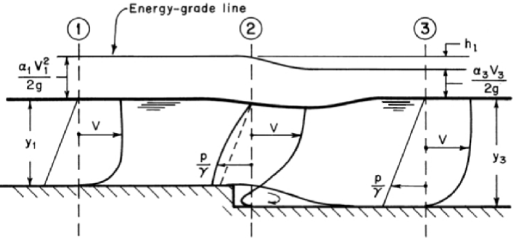
\includegraphics[width=0.8\linewidth]{fig71.png}
    \caption{Cambio abrupto en el fondo del canal.}
    \label{fig71}
\end{figure}

\subsection{Conservaci\'on de la masa}
Por definici\'on, el flujo volum\'etrico o caudal a trav\'es de una secci\'on se define como:
\begin{equation}
    Q = \int_A \mathbf{u} \cdot d\mathbf{A}
\label{eq1}
\end{equation}

donde $\mathbf{u}$ es el campo vectorial de velocidades, $d\mathbf{A}$ es el vector normal de area infinitesimal y $A$ es el area de la secci\'on. Si el flujo es aproximadamente paralelo, lo cual ocurre cuando existe presiones hidroest\'aticas, el angulo formado entre $\mathbf{u}$ y $d\mathbf{A}$ es cero, y si la velocidad es casi uniforme (velocidad media $V$), como es el caso de las secciones 1 y 2 en la figura~\ref{fig71}, la ecuaci\'on~\ref{eq1} se convierte en:
\begin{equation}
    Q = V \int_A  dA = QA
\label{eq2}
\end{equation}

La ecuaci\'on~\ref{eq1} es conocida como la ecuaci\'on de continuidad por lo que, para flujo permanente, $Q_1 = Q_3$ o $A_1 V_1  = A_3 V_3$. 

Analizando el la distribuci\'on de velocidades en 2, es notorio que existe un flujo de reversa por lo que expresar la velocidad en terminos de la velocidad media $V$ no es posible. Esto implica que el c\'alculo de $Q$ en la secci\'on 2 a partir de la ecuaci\'on~\ref{eq2} solo es posible si la distribuci\'on de velocidad representada por el vector $\mathbf{u}$  es conocida. 


\subsection{Conservaci\'on de la cantidad de movimiento}
Por definici\'on, el flujo de cantidad de movimiento  a trav\'es de una secci\'on $A$ en direcci\'on $x$ se define como: 
\begin{equation}
    m_x = \rho \int_A v_x \left( v dA \right)
\label{eq3}
\end{equation}

donde $v_x$ es la componente de la velocidad en $x$. Para evaluar la ecuaci\'on~\ref{eq3} es necesario conocer las componented en $y$ y $z$ de la velocidad. Ecuciones similares se pueden obtener para $m_y$ y $m_z$.

Considerando una velocidad uniforme en la secci\'on, el flujo de cantidad de movimiento se puede calcular como:
\begin{equation}
    m = \rho Q \left( \beta V \right)
\label{eq4}
\end{equation}
en donde $\beta$ es un coeficiente de cantidad de movimiento el cual corrige $m$ teniendo en cuenta la distribuci\'on no uniforme de la velocidad en la secci\'on. Analisando la figura~\ref{fig71}, la ecuaci\'on~\ref{eq4} puede ser utilizada para estimar $m$ en las secciones 1 y 3 pero no en la secci\'on 1. 

La fuerza actuante sobre una secci\'on puede ser obtenida a partir de la ecuaci\'on~\ref{eq4} siempre y cuando la presi\'on en la secci\'on sea hidroest\'atica como es el caso de las secciones 1 y 3. Para el caso de la secci\'on 2 en donde no es posible determinar la fuerza  a menos que la funci\'on de distribuci\'on de presiones sea conocida, lo cual puede lograrse a trav\'es de mediciones en el labotorio.  Esto hace que la aplicaci\'on de la cantidad de movimiento en FRV sea complicada. 


\subsection{Conservaci\'on de la energ\'ia}
La energ\'ia total en una secci\'on de flujo en donde la presi\'on es hidroest\'atica se expresa como:
\begin{equation}
    H = z + y + \alpha \frac{V^2}{2g}
\label{eq5}
\end{equation}

En secciones en donde la presi\'on no es hidroest\'atica la ecuaci\'on anterior no aplica. En terminos generales, el flujo de energ\'ia en una secci\'on se expresa como:
\begin{equation}
    P = \rho g \int_A \left( z + \frac{p}{\gamma} + \frac{v^2}{2g} \right) v dA
\label{eq6}
\end{equation}

Para solucionar la ecuaci\'on anterior, la distribuci\'on de velocidades ($v$) y de presiones ($p$) debe ser conocida.

En resumen, no es posible utilizar el concepto de velocidad media o de presiones hidroest\'aticas para FRV, por lo que es necesario conocer la distribuci\'on de velocidades ($v$) y de presiones ($p$). Esto quiere decir que las leyes de conservaci\'on, como han sido comunmente aplicadas, no son posibles para FRV. Distribuciones teoricas de la velocidad como la de Bousinessq y la de Fawer pueden ser empleadas. Sin embargo en un canal en donde se presentan FGV y FRV, es preferible hacer el analisis en regiones en donde FRV no este presente. 

\section{Transiciones en canales}

Una transici\'on es un cambio local en las caracter\'isticas del canal, usualmente, cambio en el \'area , forma o direcci\'on del canal, que resulta en un cambio de estado en el flujo. Transiciones t\'ipicas son las expansiones, las contracciones y las curvas. Aquellas transiciones en donde se obtenga una relaci\'on $y=f(Q)$ se conoce como un \emph{control}; all\'i ocurre la profundidad cr\'itica. Un \emph{control artificial} ocurre en  la entrada de \emph{aliviaderos} o en la cresta de \emph{vertederos}. Por otro lado un \emph{control natural} es aquel que se presenta en la descarga libre de un canal. 

A parte de servir como estructuras para cambiar el alineamiento y/o la secci\'on transversal de un canal, las transiciones son tambi\'en diseñadas para minimizar la p\'erdida de energ\'ia, para disipar energ\'ia o para reducir la velocidad del flujo y evitar erosi\'on. Teniendo en cuenta la relacion un\'ivoca $y=f(Q)$, las transiciones tambi\'en se usan para medir el $Q$. 

\subsection{Caracter\'isticas generales}
El diseño y construcci\'on de transiciones require:
\begin{itemize}
\item Con el fin de minimizar costos y por facilidad constructiva, las transiciones deben ser simples y pueden tener fronteras discontinuas.
\item Si es necesario minimizar las p\'erdidas de energ\'ia, la transici\'on debe ser gradual y no deben existir discontinuidades en los bordes. Diseños de este tipo previenen la formaci\'on de remolinos y la separaci\'on del flujo reduciendo la posibilidad de \emph{cavitaci\'on}.
\item Las transiciones causan aceleraci\'on o desaceleraci\'on del flujo en una distancia relativamente corta y dominan el movimiento por encima de los esfuerzos cortantes en las fronteras. Esto implica que el flujo no se 1D, que las lineas de flujo se curven y que exista separaci\'on del flujo. 
\item En flujo con fuerte aceleraci\'on vertical, la velocidad y la presi\'on no solo cambian en la direcci\'on del flujo si no  tambi\'en en la vertical lo cual da lugar a flujos 2D o 3D.
\item La p\'erdida de energ\'ia en una transici\'on es despreciable y el flujo se asume irrotacional. 
\item Durante el diseño de una transici\'on, es necesario evitar la ocurrencia de ca\'idas de presi\'on (e.g. cavitaci\'on) o aumentos de presi\'on que pueden causar vibraciones e inestabilidades. 
\item Para el an\'alisis de flujo en transiciones, la distribuci\'on de velocidades es generalmente no uniforme y es posible tener velocidades negat\'ivas en partes de la secci\'on. Esto hace que sea dif\'icil calcular, por ejemplo, la energ\'ia total en la secci\'on.
\end{itemize}

\subsection{Flujo subcr\'itico}
\subsubsection{Expansiones}
Una expansi\'on ocurre por un incremento en el ancho del canal, una ca\'ida del fondo o una combinaci\'on de ambos (ver figura~\ref{fig72})
% Chau fig 7-2
\begin{figure}[h]
    \centering
    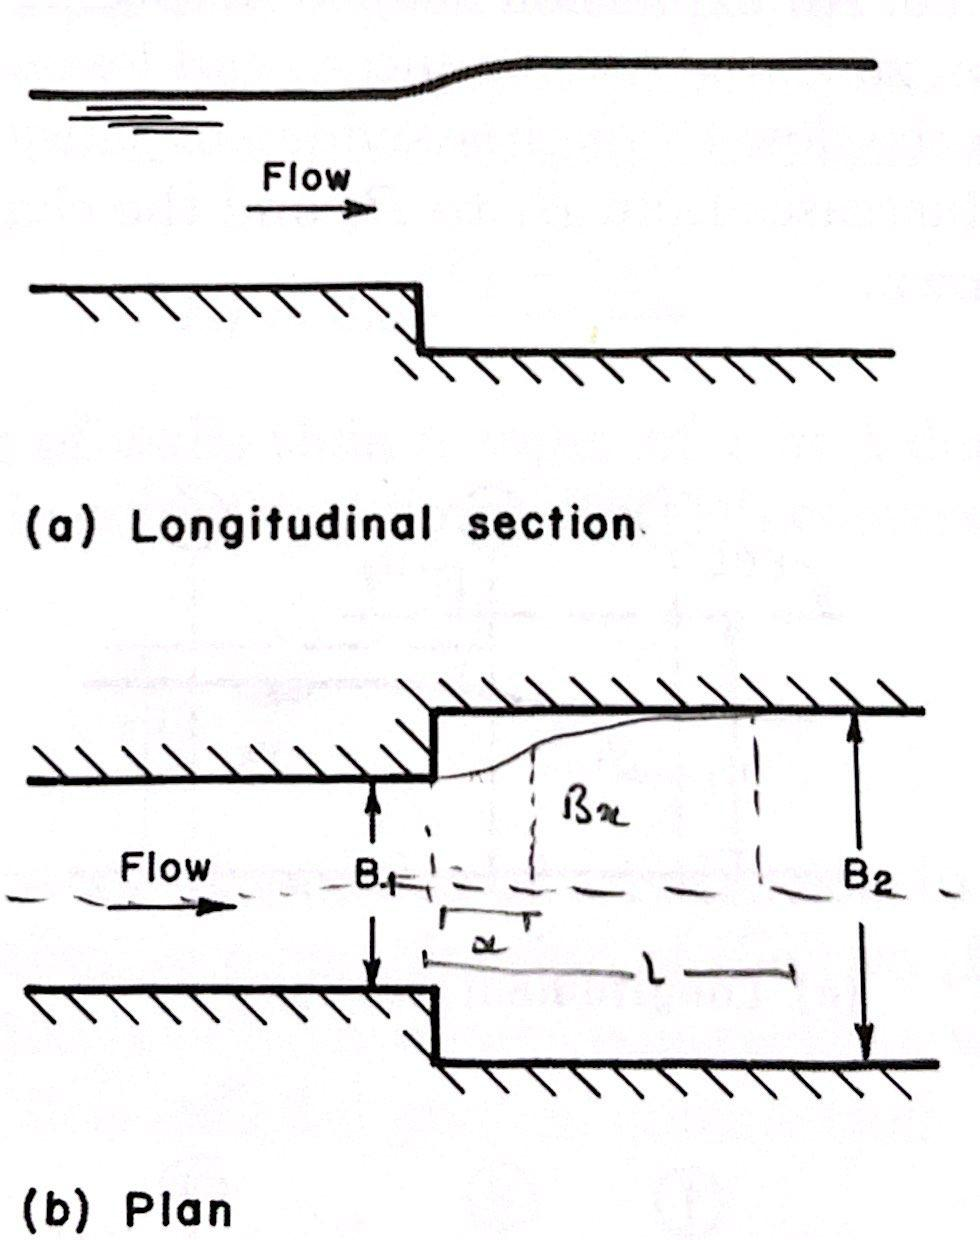
\includegraphics[width=0.8\linewidth]{fig72.jpeg}
    \caption{Expansi\'on en un canal.}
    \label{fig72}
\end{figure}

Las expansiones pueden ser abruptas (ver figura~\ref{fig72}) o graduales. Estas estructuras est\'an presentes en canales, descargas, sifones y acueductos. El diseño de expansiones requiere la selecci\'on de la forma para evitar separaci\'on de flujo y minimizar p\'erdida de energi\'a. Los criterios de diseño de expansiones se apoya en an\'alisis experimentales. Algunos hallasgos:
\begin{itemize}
    \item Se ha encontrado que el flujo aguas abajo de la expansi\'on es asim\'etrico cuando $\frac{B_2}{B_1} \leq 1.5$, donde $B_1$ es el ancho aguas arriba y $B_2$ es el ancho aguas abajo de la expansi\'on. 
    \item La forma de una linea de flujo a trav\'es de una expansi\'on se puede representar por la siguiente ecuaci\'on:
    \begin{equation}
        \frac{B_x - B_1}{B_2 - B_1} = \frac{x}{L} \left[ 1- \left(1-\frac{x}{L}\right)^m \right]
        \label{eq1}
    \end{equation}
    en donde $B_x$ es dos veces la distancia desde el eje de simetr\'ia de la expansi\'on a la l\'inea de flujo mas externa, $x$ es la distancia horizontal a lo largo del eje de simetr\'ia desde donde inicia la expansi\'on, $L$ es la distancia horizontal a lo largo del eje de simetr\'ia donde la linea de flujo toca la frontera y $m$ es un exponente que varia como $0.6\leq m \leq 0.66$. 
    
    Al diseñar la forma de una expansi\'on siguiendo la ecuacion anterior, se garantiza la menor separaci\'on de flujo y se minimizan las p\'erdidas de energ\'ia. 
\end{itemize}

Consideremos la expansi\'on repentina mostrada en la figura~\ref{fig73} en donde se cambia de manera abrupta de un ancho $B_1$ a $B_2$.
% Chau fig 7-3
\begin{figure}[h]
    \centering
    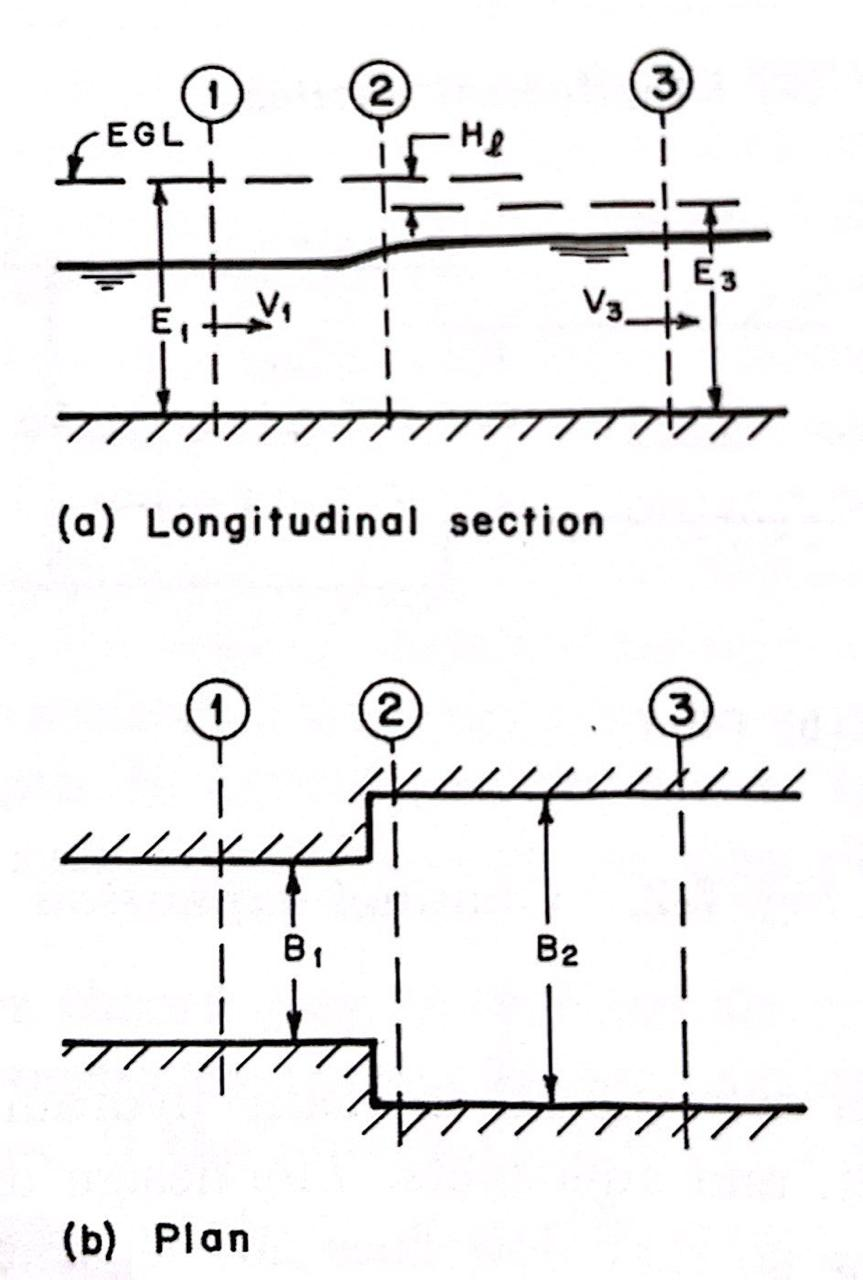
\includegraphics[width=0.8\linewidth]{fig73.jpeg}
    \caption{Expansi\'on en un canal.}
    \label{fig73}
\end{figure}

Si se asume que: 1) $E_2 = E_1$, 2) $F_{s_1} = F_{s_2}$, 3) $y_1 = y_2$, 4) $B_2 \approx B_1$ y 5) $Fr_1^n \approx 0$ para $n \ge 4$, se puede demostrar que:
\begin{equation}
    E_1 - E_3 = \frac{V_1^2}{2g}\left[ \left( 1- \frac{B_1}{B_2}\right)^2 + 2Fr_1^2 \left(B_2 - B_1\right)\frac{B_1^3}{B_2^4}\right]
    \label{eq2}
\end{equation}
En la ecuaci\'on anterior, el segundo termino dentro de los parentesis es despreciables si $Fr_1 < 0.5$ o si $B_2 / B_1 > 1.5$. En muchas aplicaciones, la condici\'on  $B_2 / B_1 > 1.5$ se cumple. Para el caso en que $B_2 / B_1 < 1.5$ las p\'erdidas de energ\'ia en la expansion son despreciables. 

En terminos generales las p\'erdidas de energ\'ia en una expansi\'on subita, se calcula como:
\begin{equation}
    H_l = \frac{\left( V_1 - V_3 \right)^2}{2g}
    \label{eq3}
\end{equation}
An\'alisis experimentales han demonstrado que la ecuaci\'on anterior sobre-estiman las p\'erdidas de energ\'ia en cerca de un 10\%.

En expansiones graduales cuyos bordes cambian como 4H:1V, las p\'erdidas de energ\'ia son:
\begin{equation}
    H_l = 0.3\frac{\left( V_1 - V_3 \right)^2}{2g}
    \label{eq4}
\end{equation}
Para transiciones m\'as graduales, las p\'erdidas no son significativamente menores a las estimadas en la ecuaci\'on~\ref{eq4}, sin embargo, los costos pueden aumentar sustancialmente.

\subsubsection{Contracciones}
Las contracciones en un canal se presentan cuando el ancho del canal se reduce, cuando el fondo del canal aumenta o como una combinaci\'on de ambas (ver figura~\ref{fig74}). 
% Chau fig 7-4
\begin{figure}[h]
    \centering
    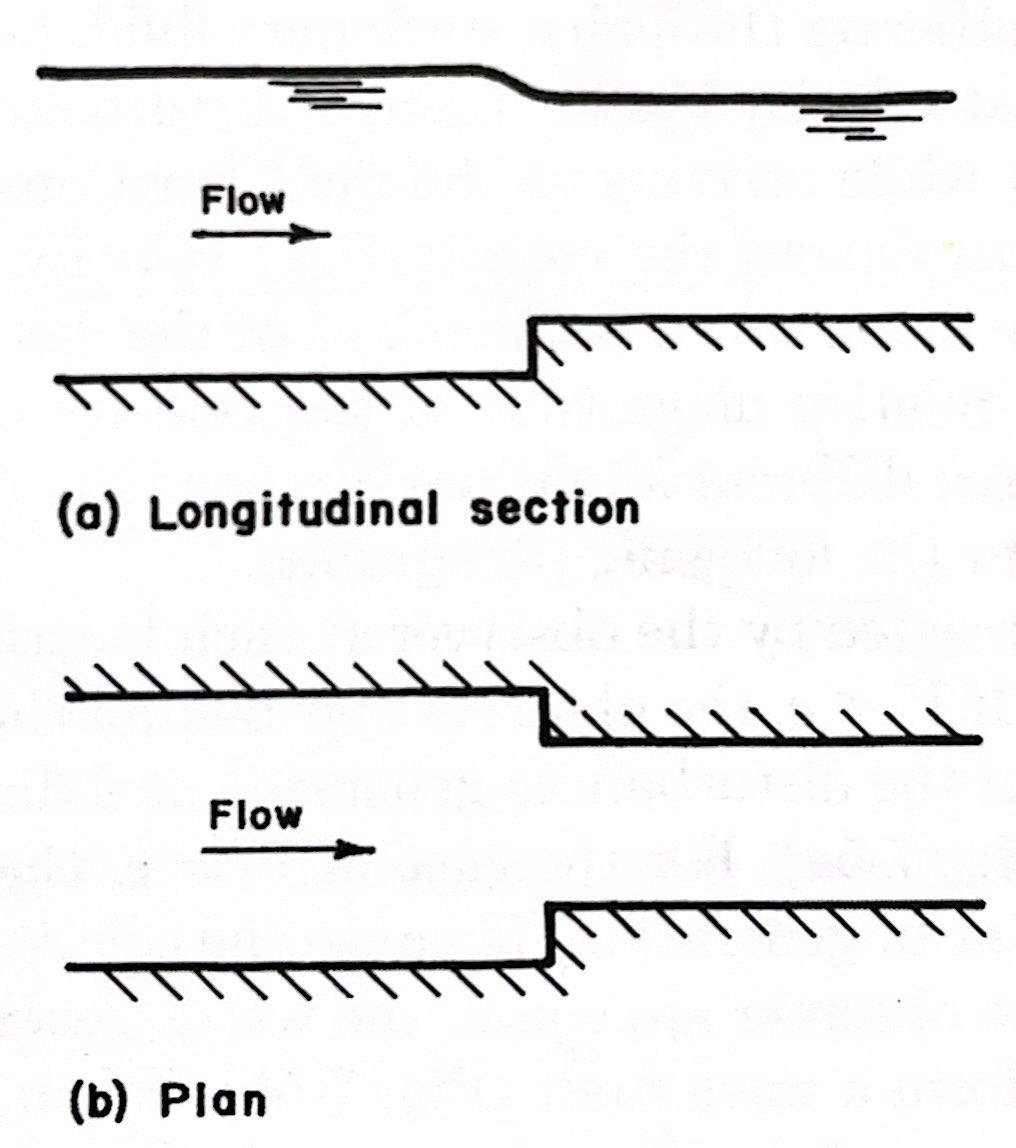
\includegraphics[width=0.8\linewidth]{fig74.jpeg}
    \caption{Contracci\'on en un canal.}
    \label{fig74}
\end{figure}
Existen contracciones abruptas y graduales. An\'alisis experimentales han demonstrado que las p\'erdidas de energ\'ia en una contracci\'on son menores que las presentes en una expansi\'on, y son iguales a:
\begin{equation}
    H_l = 0.23\frac{V_3^2}{2g}
    \label{eq5}
\end{equation}
La ecuaci\'on~\ref{eq5} aplica para contracciones abruptas. Para contracciones con bordes redondeados, la p\'erdida de energ\'ia se calcula como:
\begin{equation}
    H_l = 0.11\frac{V_3^2}{2g}
    \label{eq5}
\end{equation}
Note que $V_3$ es la velocidad en la seccion de flujo de mayor contracci\'on (aguas abajo de la contracci\'on) en donde la velocidad es c\'asi uniforme. Otros autores han econtrado que la perdidas de energ\'ia se calculan como:
\begin{equation}
    H_l = C\frac{V_3^2}{2g}
    \label{eq5}
\end{equation}
donde $C=0.35$ para bordes cuadrados y $C=0.18$ para bordes redondeados. 

Contracciones muy fuertes pueden causar condiciones criticas del flujo en la contracci\'on o que la energ\'ia aguas arriba no sea suficiente para pasar a trav\'es de la contracci\'on. 

\subsection{Supercritical flow}
El flujo supercr\'itico a trav\'es de transiciones puede ser problem\'atico porque es com\'un la formaci\'on de ondas de choque en la superficie del flujo. Las ondas de choque son cambios repentinos de la profundidad y de la velocidad que se producen por cambios dr\'asticos en las condiciones de flujo. 

Para analisar las ondas de choque imaginemos un observador que viaja sobre un fluido cuya velocidad es $V$  y causa una perturbaci\'on (e.g. cambios en el alineamiento del canal, irregularidades en en la superficie de la pared, etc). La celeridad de una onda, se define como $c$, la cual es la velocidad relativa con la cual viaja la perturbaci\'on en el flujo. Dependiendo de la magnitud de $V$ y $c$ existen tres situaciones posibles  que se observan en la figura~\ref{fig75}.
% Chau fig 7-5
\begin{figure}[h]
    \centering
    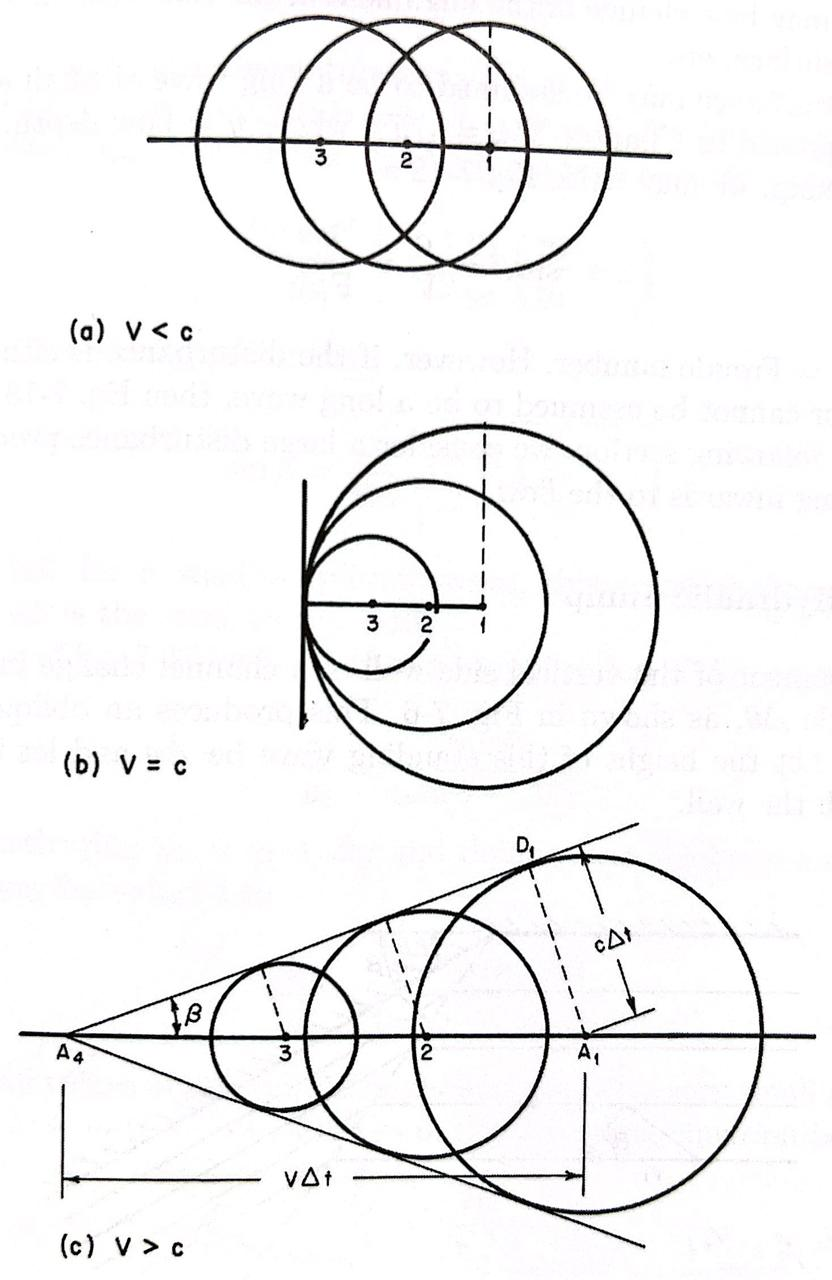
\includegraphics[width=0.8\linewidth]{fig75.jpeg}
    \caption{Propagaci\'on de una perturbaci\'on.}
    \label{fig75}
\end{figure}
Analizando el caso $V>c$, es posible encontrar una relaci\'on entre $V$, $c$ y $\beta$:
\begin{equation}
    \sin \beta = \frac{A_1 D_1}{A_1 A_4} = \frac{c \Delta t}{V \Delta t} = \frac{c}{V}
    \label{eq6}
\end{equation}

En el caso de ondas largas de pequeña amplitud $c = \sqrt{gy}$, donde $y$ es la profundidad de flujo. Reemplazando en la ecuaci\'on~\ref{eq6}, se tiene:
\begin{equation}
    \sin \beta =  \frac{c}{V} = \frac{1}{Fr}
    \label{eq6}
\end{equation}

\subsubsection{Resalto hidr\'aulico oblicuo}
En el caso de un flujo supercr\'itico que pasa a trav\'es de una contracci\'on gradual en un canal rectangular, se generan ondas de gran magnitud debido a la deflexi\'on de las lineas de flujo hacia adentro dando lugar a la ocurrencia de resaltos hidr\'aulicos oblicuos (ver figura~\ref{fig76}). 
% Chau fig 7-6
\begin{figure}[h]
    \centering
    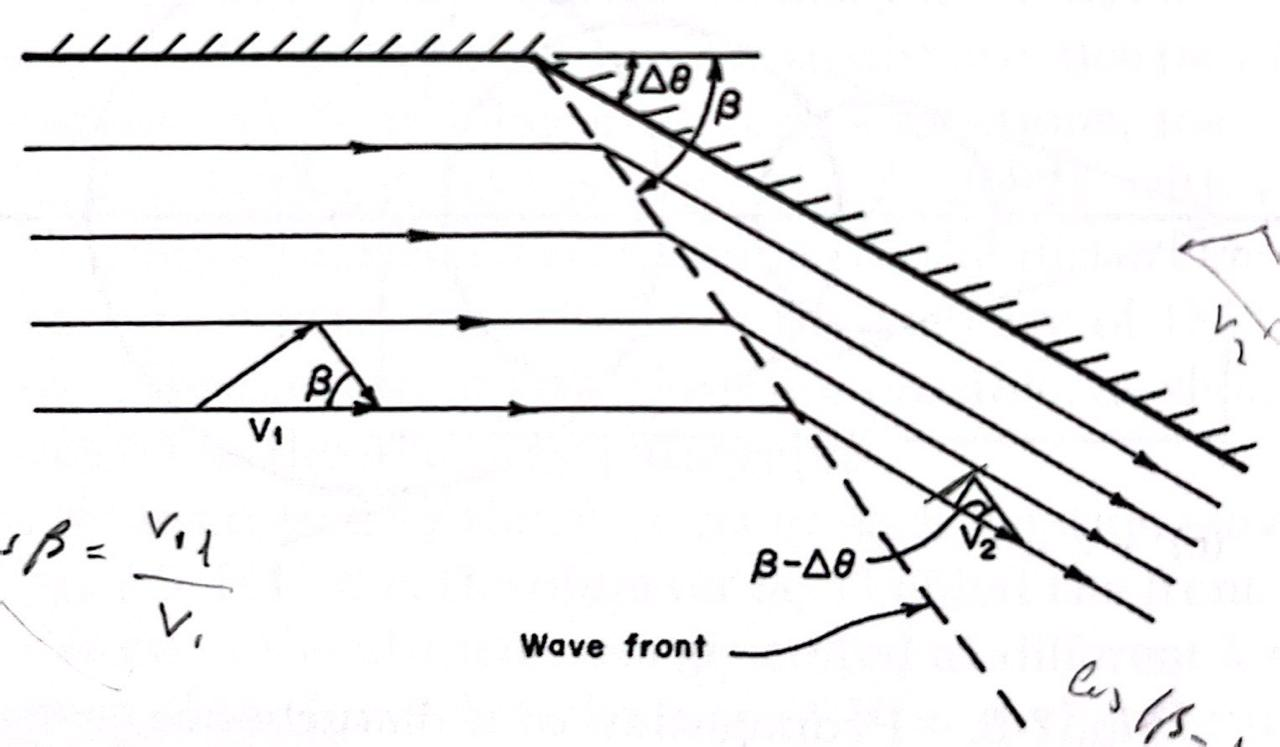
\includegraphics[width=0.8\linewidth]{fig76.jpeg}
    \caption{Resalto hidr\'aulico oblicuo.}
    \label{fig76}
\end{figure}

Analizando la figura~\ref{fig76}, las velocidades tangenciales antes y despues de la contracci\'on (frente de onda) deben ser iguales:
\begin{equation}
   V_1 \cos \beta = V_2 \cos \left(\beta - \Delta \theta \right)
    \label{eq6a}
\end{equation}

donde $V_1$ es la velocidad antes de la contracci\'on, $V_2$ es la velocidad en la contracci\'on, $\Delta \theta$ es el angulo de la contracci\'on y $\beta$ es el anue forma el )rente de onda con la horizontal. 

A partir de la ecuacion de continuidad y de las velocidades perpendiculares al frente de onda, se tiene:
\begin{equation}
   y_1 V_1 \sin \theta = y_2 V_2 \sin \left(\beta - \Delta \theta \right)
    \label{eq7}
\end{equation}

De la conservaci\'on de cantidad de movimiento para la velocidad perpendicular $V_1 \sin \beta$, se tiene:
\begin{equation}
    \frac{V_1 \sin^2 \beta}{gy_1} = \frac{1}{2}\frac{y_2}{y_1}\left( \frac{y_2}{y_1} + 1 \right)
    \label{eq8}
\end{equation}
De esta ecuaci\'on se tiene:
\begin{equation}
    \sin \beta = \frac{1}{Fr_1}\sqrt{\frac{1}{2}\frac{y_2}{y_1}\left( \frac{y_2}{y_1} + 1 \right)}
    \label{eq9}
\end{equation}
Note que para ondas de pequeña amplitud, la ecuaci\'on~\ref{eq9} se convierte en la ecuaci\'on~\ref{eq6}.

Dividiendo la ecuaci\'on~\ref{eq7} por la ecuaci\'on~\ref{eq6a}, se tiene:

\begin{equation}
    \frac{y_2}{y_1} = \frac{\tan \beta}{\tan \left(\beta-\Delta \theta \right)}
    \label{eq10}
\end{equation}
Sustituyendo $y_2 = y_1 + \Delta y$, donde $\Delta y$ es la altura de la onda, en la ecuaci\'on~\ref{eq10}, se tiene:
\begin{equation}
    \frac{\Delta y}{y} = \frac{\sec^2 \beta \tan \Delta \theta}{\tan \beta - \tan \Delta \theta}
    \label{eq11}
\end{equation}

Para valores pequeños de $\Delta \theta$, $\tan \theta \approx \Delta \theta$ y $\tan \Delta \theta$ es muy pequeño con respecto a $\tan \beta$. Aplicando l\'imites cuando $\Delta \theta \rightarrow 0$, la ecuaci\'on~\ref{eq12} se convierte en:
\begin{equation}
    \frac{dy}{d\theta} = \frac{2y}{\sin 2\beta}
    \label{eq12}
\end{equation}
Combinando las ecuaciones ~\ref{eq6} y ~\ref{eq12}, se tiene:
\begin{equation}
    \frac{dy}{d\theta} = \frac{V^2}{g}\tan \beta
    \label{eq13}
\end{equation}
La ecuaci\'on~\ref{eq13} define la variaci\'on de la profundidad de flujo en la transici\'on. Esta ecuaci\'on indica que $y$ cambia en funci\'on de $\theta$ a lo largo del frente de onda oblicuo.

Teniendo en cuenta que las p\'erdidas de energ\'ia pueden son despreciables, la velocidad se puede expresar como $V = \sqrt{2g\left(E-y\right)}$. Reemplazando esta expresi\'on en la ecuaci\'on~\ref{eq13} y utilizando la ecuaci\'on~\ref{eq6}, se tiene:
\begin{equation}
    \frac{dy}{d\theta} = \frac{2\left(E-y\right)\sqrt{y}}{\sqrt{2E-3y}}
    \label{eq14}
\end{equation}

Integrando la ecuaci\'on~\ref{eq14} y sustituyendo $E$ en terminos de $y$ y de $Fr$, se tiene:
\begin{equation}
   \theta = \sqrt{3}\tan^{-1} \frac{\sqrt{3}}{\sqrt{Fr^2 - 1}} - \tan^{-1} \frac{1}{\sqrt{Fr^2 -1}} + \theta_0
    \label{eq15}
\end{equation}
donde $\theta_0$ es la constante de integraci\'on la cual se obtiene sustituyendo $\theta = 0$ para la profundidad $y = y_1$. Esta ecuaci\'on estima los cambios en las profundidades en la transici\'on debido a cambios de $\theta$. 

\section{Vertederos}
Los \emph{vertederos} son estructuras hidraulicas usadas en el laboratorio para medir el caudal en canales artificiales o naturales. Existen dos tipos de vertederos: 1) \emph{vertederos de cresta delgada} y 2) \emph{vertederos de cresta ancha}. 

\subsection{Vertedero de cresta delgada}
Esta compuesto por una lamina delgada que es empotrada perpendicular a la direcci\'on del flujo en las paredes y al fondo del canal. La parte superior de la placa tiene una abertura, usualmente, rectangular, triangular o trapezoidal cuyo bordes son afilados para garantizar un paso del agua sin perturbaciones a trav\'es de la abertura. En el caso de vertederos triangulares, estos son usados para caudales pequeños. El analisis teorico del flujo sobre un vertedero considera que el flujo esta en contacto con la presi\'on atmosferica arriba y abajo del chorro que atraviesa el vertedero.  

Consideremos el flujo sobre un vertedero rectangular como el mostrado en la figura~\ref{fig77}. 
% Chau fig 7-7
\begin{figure}[h]
    \centering
    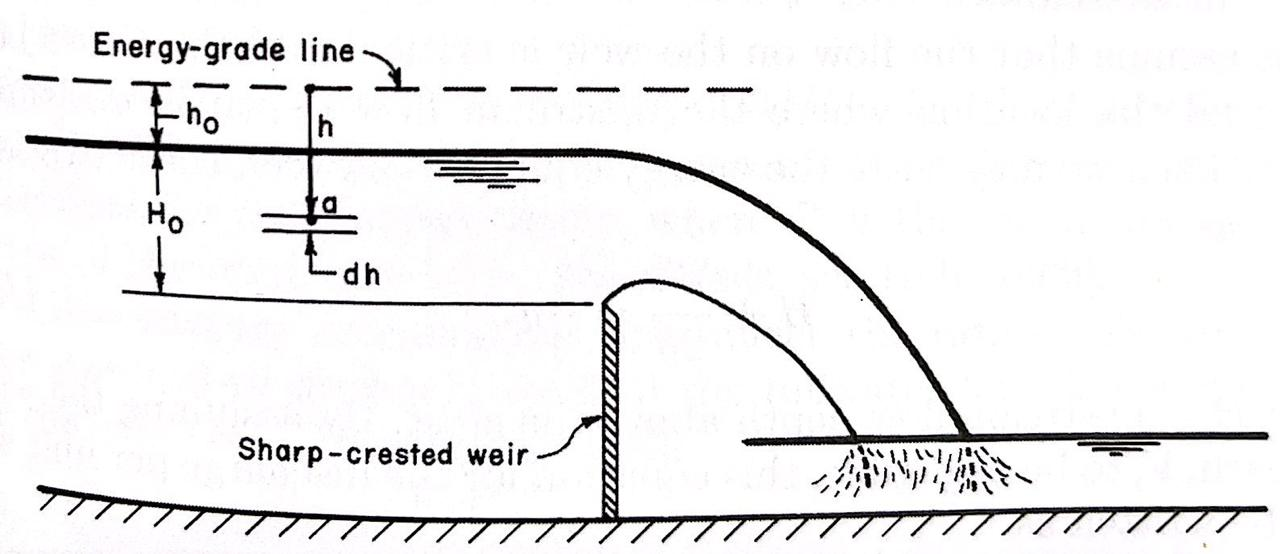
\includegraphics[width=0.8\linewidth]{fig77.jpeg}
    \caption{Vertedero rectangular de cresta delgada.}
    \label{fig77}
\end{figure}



Si se asume que cualquier punto en la \emph{lamina de agua} (nappe en Ingles), la cual es la porci\'on del flujo que fluye por encima del vertedero, la presi\'on es igual a la presi\'on almosferica, la energia en el punto $a$ de la figura es $h = \frac{P_{atm}}{\gamma} + \alpha \frac{V^2}{2g} \approx \alpha \frac{V^2}{2g}$, donde $h$ es la energ\'ia en el punto $a$. Despejando la velocidad, se tiene que $V = \sqrt{2 \alpha g h }$. En analisis experimentales, se ha encontrado que $\alpha \approx 1$ en vertederos. El caudal por unidad de ancho $q$ se puede calcular como:
\begin{equation}
    %q = \int_{h_o}^{H_o + h_o} \sqrt{2gh} dh = \frac{2}{3}\sqrt{2g}\left[ \left(H_o + h_o \right)^{3/2} - \left( h_o \right)^{3/2} \right]
    q = \int_{0}^{H_o} \sqrt{2gh} dh = \frac{2}{3}\sqrt{2g}\left(H_o \right)^{3/2}
    \label{eq16}
\end{equation}
Teniendo en cuenta contracciones del flujo y otros efectos, se introduce el coeficiente de correcci\'on de caudal $C_d$, por lo que la ecuaci\'on~\ref{eq16} queda:
\begin{equation}
    q = \frac{2}{3}C_d\sqrt{2g}\left(H_o \right)^{3/2}
    \label{eq17}
\end{equation}
Para un verderdo cuyo ancho de cresta es $B$, el caudal queda expresado como:
\begin{equation}
    Q = \frac{2}{3}C_d B\sqrt{2g}\left(H_o \right)^{3/2}
    \label{eq17a}
\end{equation}
Para vertederos rectangulares con contracciones, $Q$ se expresa como:
\begin{equation}
    Q = \frac{2}{3}C_d B' \sqrt{2g}\left(H_o \right)^{3/2}
    \label{eq17b}
\end{equation}
donde $B' = B - a$ y $a$ es el ancho ocupado por las contracciones. 

Con base en resultados experimentales:
\begin{equation}
    C_d = 0.611 + 0.08\frac{H_o}{P}
    \label{eq18}
\end{equation}
donde $P$ es la distance vertical a la cresta del vertedero desde el fondo del canal. Esta formula es valida para $H_o / P < 5$. Para $H_o / P > 15$ la cresta del vertedero queda sumergida y el vertedero deja de controlar el flujo de manera efectiva y el caudales se puede calcular a partir de la relaci\'on de flujo cr\'itico por lo que se asume que $y_c = H_o$.

Para vertederos triangulares conocidos como vertederos \emph{v-notch}, se tiene que:
\begin{equation}
    Q = \int_A \sqrt{2gh} dA = \sqrt{2g} \int_A \sqrt{h} dh dx = \sqrt{2g} \int_0^{H_o} \sqrt{h} dh \left(H_o-h\right) \tan \left(\frac{\alpha}{2}\right) = \frac{8}{15} \tan\left(\frac{\alpha}{2}\right) \sqrt{2g} H_o^{5/2}
    \label{eq19}
\end{equation}
donde $\alpha$ es el angulo del vertedero triangular. Teniendo en cuenta las contracciones, el caudal se puede corregir y expresar como:
\begin{equation}
    Q =  \frac{8}{15} C_d \tan\left(\frac{\alpha}{2}\right) \sqrt{2g} H_o^{5/2}
    \label{eq20}
\end{equation} 
Para $\alpha = 90^o$, se ha encontrado que $C_d \approx 0.585$, por lo que reemplanzado estos valores en la ecuaci\'on anterior se tiene:
\begin{equation}
    Q =  1.4 H_o^{5/2}
    \label{eq20a}
\end{equation} 

Para vertederos trapezoidales, sumando   las ecuaciones ~\ref{eq17b} y ~\ref{eq20}, se tiene:
\begin{equation}
    Q =  \frac{2}{3}C_d B' \sqrt{2g}\left(H_o \right)^{3/2} + \frac{8}{15} C_d \tan\left(\frac{\alpha}{2}\right) \sqrt{2g} H_o^{5/2}
    \label{eq21}
\end{equation}

\section{Vertederos de cresta ancha}
Los vertederos de cresta ancho son estructuras en donde el fondo del canal se eleva brusca o gradualmente por una longitud finita. Esta elevaci\'on del fondo al prolongarse por cierto distancia da origen a un flujo paralelo al vertedero en donde suele presentarse la profundidad cr\'itica $y_c$. De acuerdo con esto, estos vertederos tambien pueden ser usados para determinar el caudal, en este caso, en funcion de $y_c$.

Analisando el vertedero en un canal rectangular de la figura~\ref{fig78} en donde ocurre la profundidad cr\'itica en la cresta y, teniendo en cuenta que las p\'erdidas de energ\'ia son despreciales entre una secci\'on antes del vertedero y la secci\'on donde ocurre $y_c$, el balance de energ\'ia entre las secciones es:
% Chau fig 7-8
\begin{figure}[h]
    \centering
    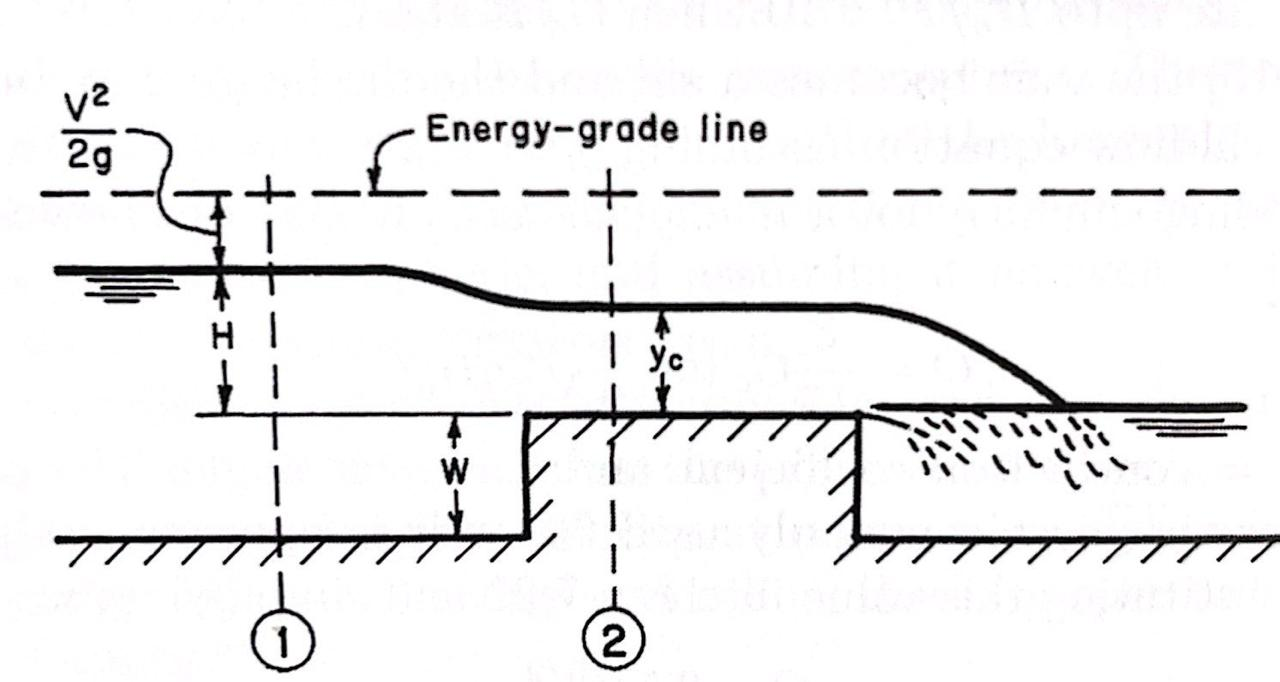
\includegraphics[width=0.8\linewidth]{fig78.jpeg}
    \caption{Vertedero de cresta ancha.}
    \label{fig78}
\end{figure}

\begin{equation}
    H + \frac{V^2}{2g} = E_c = \frac{3}{2}y_c
    \label{eq22}
\end{equation}
donde $H$ es la profundidad aguas arriba del vertedero.

Si se asume que la velocidad de aproximaci\'on $V$ es despreciable en la ecuaci\'on anterior, se tiene que $y_c = \frac{2}{3}H$. Teniendo en cuenta que $q = \sqrt{g y_c^3}$, se tiene que el caudal por unidad de ancho $q$ es:

\begin{equation}
    q = \frac{2}{3}H \sqrt{\frac{2}{3} g H}
    \label{eq23}
\end{equation}
Para un canal de ancho $B$ y teniendo en cuenta otras consideraciones, el caudal se calcula como:
\begin{equation}
    Q = C B \sqrt{g} H^{3/2}
    \label{eq24}
\end{equation}
donde $C$ es un coeficiente de correcci\'on del $Q$. 

Si $W$ es la altura del vertedero, $V = \frac{Q}{\left[B\left(H+W\right)\right]}$. Utilizando las ecuaciones ~\ref{eq22} y ~\ref{eq24}, se tiene:
\begin{equation}
    \frac{H}{H+W} = \frac{\left[3 C^{2/3}-2 \right]^{1/2}}{C}
    \label{eq25}
\end{equation}

Analizando la longitud del vertedero $L$, el vertedero se considere largo si $L/H >3$. Si esta condici\'on se cumple es necesario reducir $H$ en una cantidad $\delta^*$ con el fin de tener en cuenta los efectos viscosos.

En vertederos de cresta ancha, la sumergencia aguas abajo del vertedero puede afectar la estimaci\'on del caudal, esto sucede cuando el nivel aguas abajo del vertedero es mayor que $0.8H$. 

\section{Aliviaderos}
Los aliviaderos son estructuras hidr\'aulicas usadas para descargar caudales de excesos en sistemas de control de inundaciones y regulaci\'on de caudales, o para descargas controladas en irrigaci\'on y navegaci\'on. Los aliviaderos se pueden clasificar con base en los siguientes criterios: funcionalidad, estructura o tipo de entrada. De acuerdo a la funci\'on que cumplan, estos pueden ser estrucutas de: servicio, auxiliare o de emergencia. Con base en su estructura, esto pueden ser aliviaderos de: excesos, sistema de conduccion, o tunneles. De acuerdo con el tipo de entrada, estos pueden ser: orificios, sifones, canales laterales y morning glory. 

\subsection{Aliviadero de excesos}
Los aliviaderos de excesos se construyen sobre el cuerpo de presas por gravedad, de arco y de contrafuerte, en donde parte del cuerpo de la presa es usado para el aliviadero. Estas estructuras estan compuestas por: la cresta, el canal y el disipador de energ\'ia. 

\subsubsection{cresta de un aliviadero de excesos}
Para el diseño de la cresta, se deben tener en cuenta las siguientes consideraciones:
\begin{itemize}
    \item La presi\'on sobre la cresta es atmosf\'erica si la forma de la cresta es igual a la forma de la parte de abajo del chorro.
    \item Puede occurrit que la presi\'on pueden ser mayor o menor que la presi\'on atmosf\'erica dependiendo de la forma de la cresta del aliviadero (ver figura~\ref{fig717}).
% Chau fig 7-17
\begin{figure}[h]
    \centering
    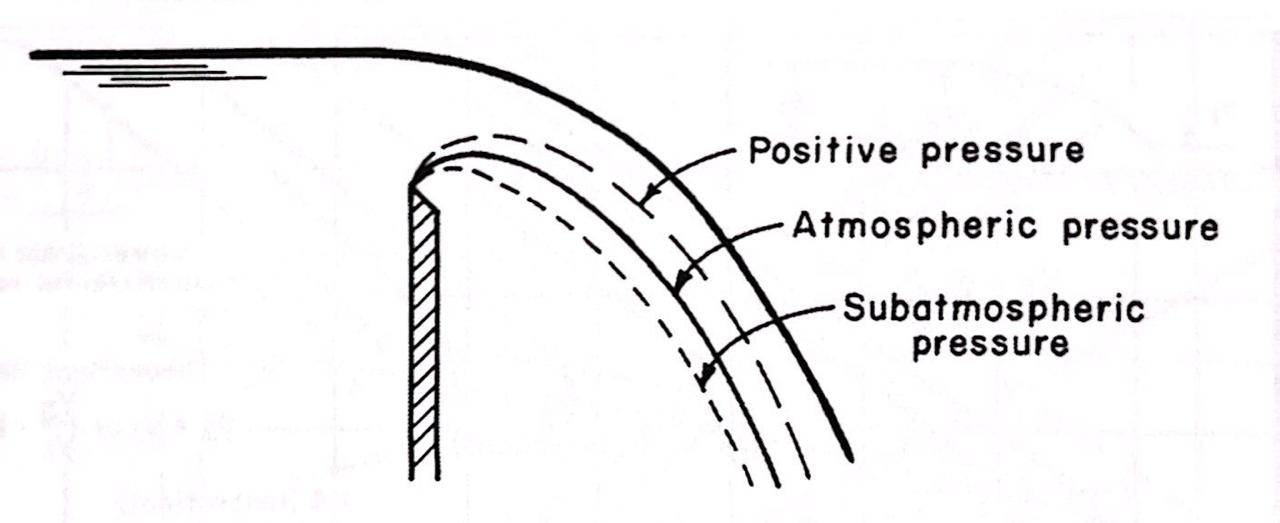
\includegraphics[width=0.8\linewidth]{fig717.jpeg}
    \caption{Presi\'on sobre un aliviadero de excesos.}
    \label{fig717}
\end{figure}

\item La forma de la cresta se basa en la  \emph{cabeza de diseño}, $H_d$, la cual es seleccionada para un sitio espec\'ifico y debe ser tal que prevenga la presi\'on m\'inima igual a -6 m con el fin de evitar cavitaci\'on. La figura~\ref{fig718} se usa para seleccionar $H_d$ de tal manera que la condici\'on de m\'inima presi\'on se satisfaga. En esta figura, $H$ es la carga m\'axima sobre sobre la cresta del aliviadero. Usualmente, $H_d$ es selecionada de la  figura~\ref{fig718} y de tal manera que  $1.3< H/H_d < 1.5$. Esto garantiza una \'optima capacidad de descarga del aliviadero y la no ocurrencia de cavitaci\'on. 
% Chau fig 7-18
\begin{figure}[h]
    \centering
    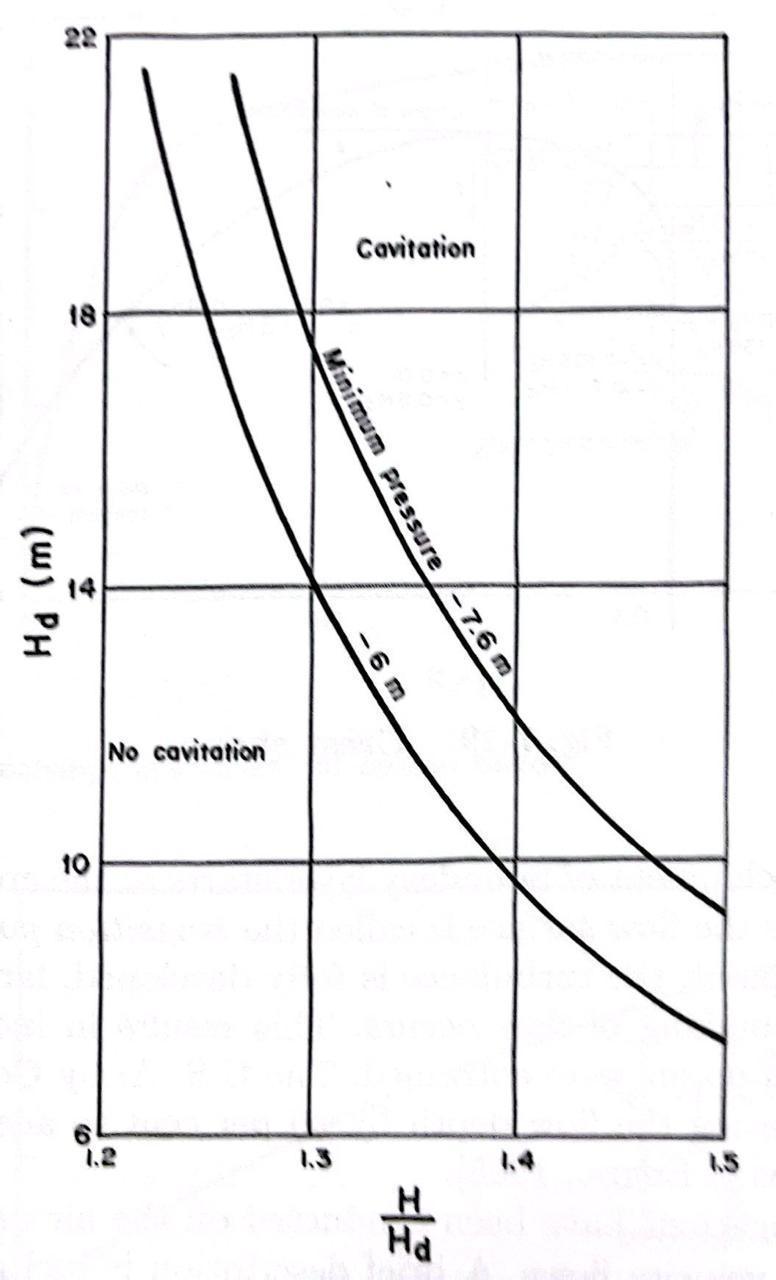
\includegraphics[width=0.8\linewidth]{fig718.jpeg}
    \caption{Cabeza de diseño para aliviaderos de excesos.}
    \label{fig718}
\end{figure}

\item La forma de la cresta puede ser determinada usando las relaciones de la figura~\ref{fig719}, las cuales fueron desarrolladas por el U.S Army Corps of Engineers basado en extensos an\'alisis de laboratorio. 
% Chau fig 7-19
\begin{figure}[h]
    \centering
    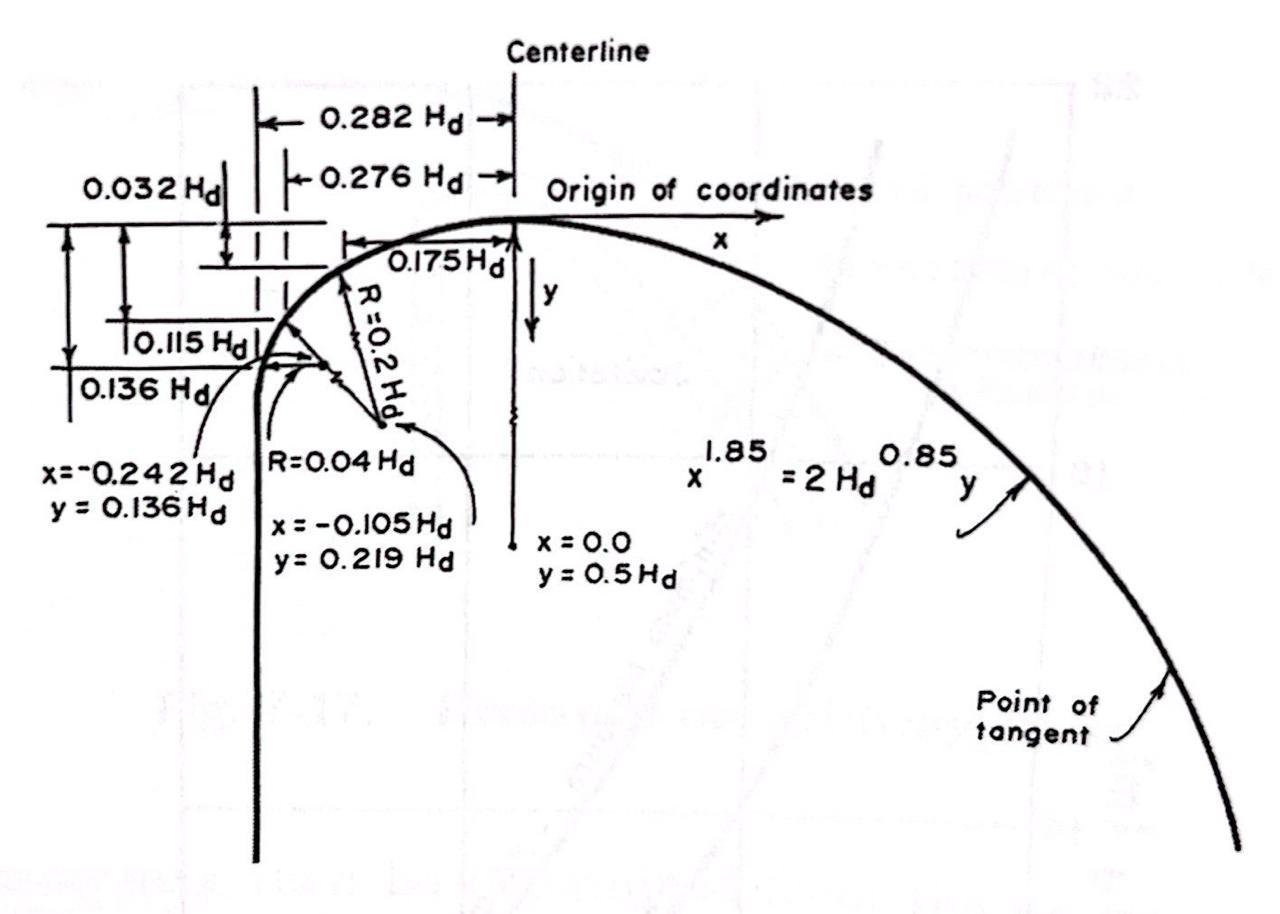
\includegraphics[width=0.8\linewidth]{fig719.jpeg}
    \caption{Forma de la cresta de un aliviadero de excesos.}
    \label{fig719}
\end{figure}
\end{itemize}

\subsubsection{Curva de calibraci\'on}
La curva de calibraci\'on en un aliviadero de excesos es la relaci\'on matem\'atica entre el nivel del embalse aguas arriba del aliviadero y el caudal que descarga el aliviadero. Esta curva, se puede escribir como:
\begin{equation}
    Q = C L_e \sqrt{2g} H_e^{1.5}
    \label{eq26}
\end{equation}
donde $L_e$ es la longitud efectiva del aliviadero, $C$ coeficiente de descarga y $H_e$ es la cabeza total de energ\'ia sobre la cresta y es $H_e = H +\frac{V_o^2}{2g}$. Normalmente la velocidad de aproximaci\'on al vertedero $V_o$ es pequeña, por lo que $H_e \approx H$.

Para determinar $C$ es necesario determinar primero $C_d$ para la $H_d$ (ver figura~\ref{fig720}a). $C$ es determinado para otro $H$ con base en la figura~\ref{fig720}b. 
% Chau fig 7-20
\begin{figure}[h]
    \centering
    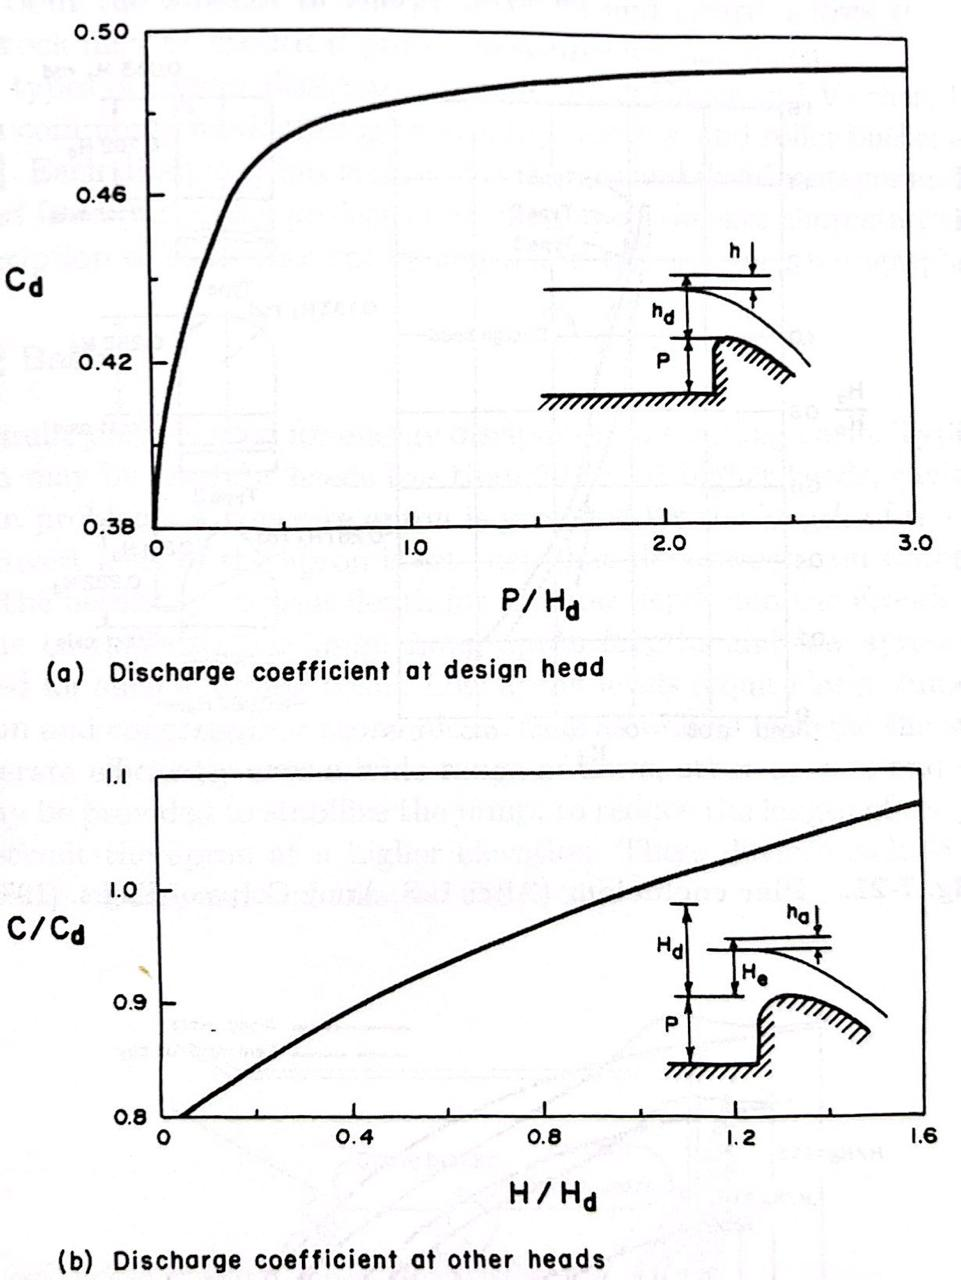
\includegraphics[width=0.8\linewidth]{fig720.jpeg}
    \caption{Coeficientes de descarga en aliviadero de excesos.}
    \label{fig720}
\end{figure}


La $L_e$, la cual es la longitud sin tener en cuenta pilas y otras estructuras, se calcula como:
\begin{equation}
    L_e = L_n - 2\left( N k_p + k_a \right) H_e 
    \label{eq27}
\end{equation}
donde $L_n$ es la longitud total del aliviadero, $k_p$ es el coeficiente de pila y $k_a$ es un coeficiente de contracci\'on por estribos. En muchos casos, $k_a$ es pequeño y puede ser despreciado. $k_p$ se determina a trav\'es de la figura~\ref{fig721}.
% Chau fig 7-21
\begin{figure}[h]
    \centering
    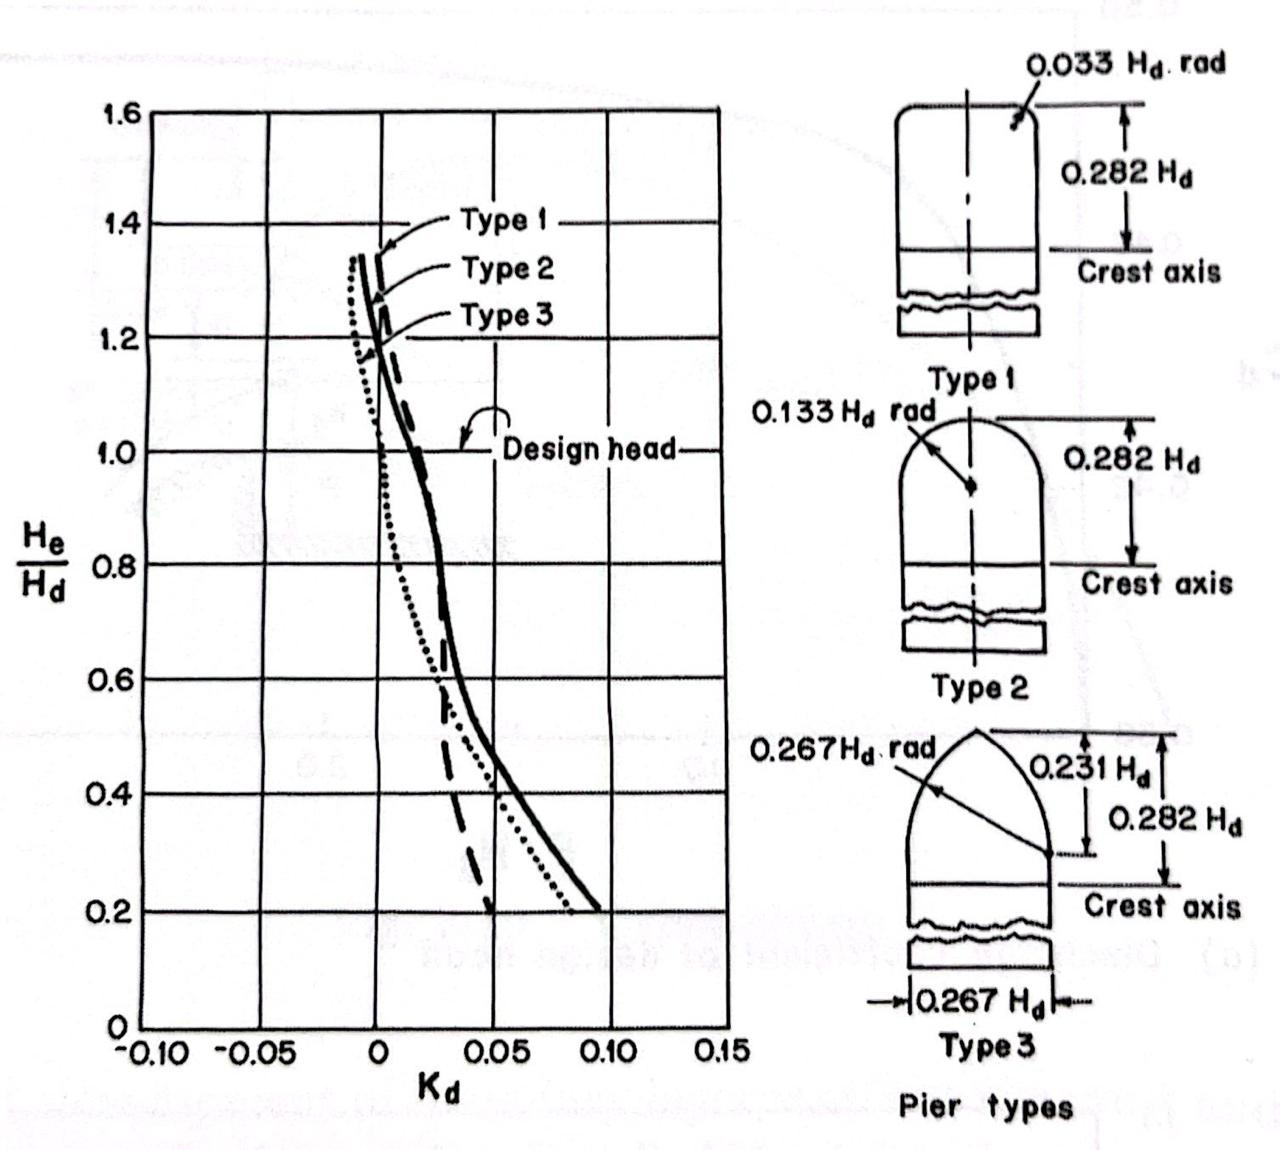
\includegraphics[width=0.8\linewidth]{fig721.jpeg}
    \caption{Coeficientes de pilas, $k_p$.}
    \label{fig721}
\end{figure}

\subsubsection{Perfil de la l\'amina de agua}
El perfil de la l\'amina de agua debe encajar entre las paredes del aliviadero (ver figura~\ref{fig722}).
% Chau fig 7-22
\begin{figure}[h]
    \centering
    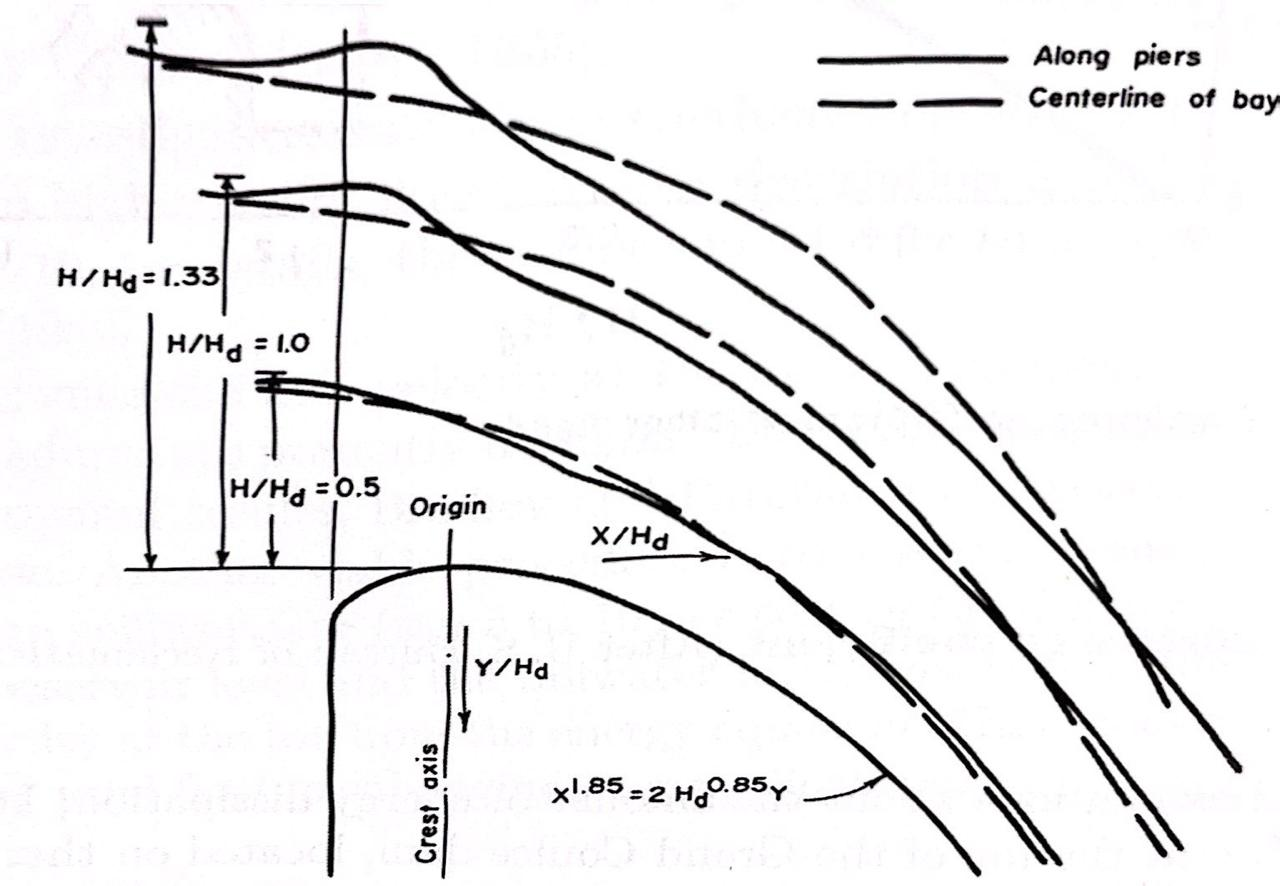
\includegraphics[width=0.8\linewidth]{fig722.jpeg}
    \caption{Perfiles de la l\'amina de agua.}
    \label{fig722}
\end{figure}

\subsubsection{Canal de descarga}
El canal de descarga tiene pendientes entre el 0.8H:1V a 0.6H:1V por lo que aguas abajo de la cresta, se presenta un flujo turbulento completamente desarrollado en donde ingresa gran cantidad de aire y por lo tanto una expansi\'on del flujo. El U.S. Army Corps of Engineers recomienda incrementar la profundidad del flujo en un 20\% para efectode diseño del canal. Un dato importante es la velocidad al final del canal, a la entrada de la estructura de disipacion. Esta se puede estimar de forma aproximada a partir de:
\begin{equation}
    z_1 + y_1 = z_2 + y_2 + frac{V_2^2}{2g} + \Delta E
    \label{eq28}
\end{equation}

donde $z_1$ es la cota de la cresta, $y_1$ es la profundidad del agua sobre la cresta, $z_2$ es la cota del fondo del canal al final, $y_2$ es la profundidad del agua al final del canal, $V$ es la velocidad del flujo al final del canal y $\Delta E$ son las p\'erdidas de energ\'ia iguales a $\Delta E = 0.05\left(z_1 + y_1 - z_2 - y_2\right)$ o $\Delta E = 0.1\left(z_1 + y_1 - z_2 - y_2\right)$. De la ecuaci\'on anterior, es posible despejar $V_2$.

\section{Culverts}
Estas son estructuras que sirven para conducir el flujo a trav\'es de un paso subterraneo como por ejemplo en el paso de una via. Estas estructuras son conductos cerrados, de forma circular o de cajon. Aparte de las p\'erdidas de energi\'ia debido a la fricci\'on dentro del \emph{culvert}, existen p\'erdidas a la entrada de este que dependen de la forma de la entrada (ver figura~\ref{fig825}).
% French fig 8-25
\begin{figure}[h]
    \centering
    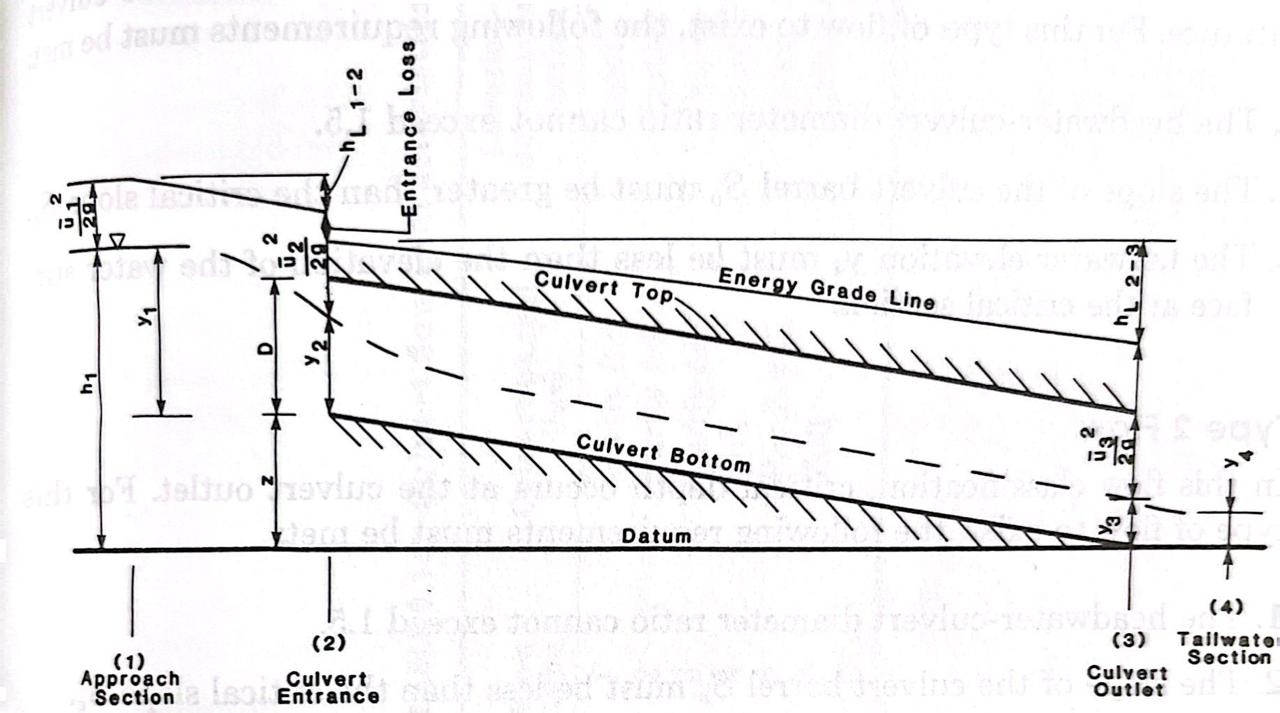
\includegraphics[width=0.8\linewidth]{fig825.jpeg}
    \caption{Flujo a trav\'es de un box-culvert (tomado de \cite{French}).}
    \label{fig825}
\end{figure}

El flujo a trav\'es de un \emph{culvert} se clasifica en seis tipos dependiendo de el nivel del flujo antes y despu\'es de la estructura (ver figura~\ref{fig826}). Note que en esta figura: $D$ es la m\'axima dimension vertical del culvert, $y_1$ es la profundidad del flujo aguas arriba del culvert, $y_c$ es la profundidad cr\'itica, $z$ es la altura de el fondo del culvert a la entrada con respecto al nivel del fondo en la salida, y $y_4$ es la profundidad del flujo aguas abajo del culvert. 
% French fig 8-26
\begin{figure}[h]
    \centering
    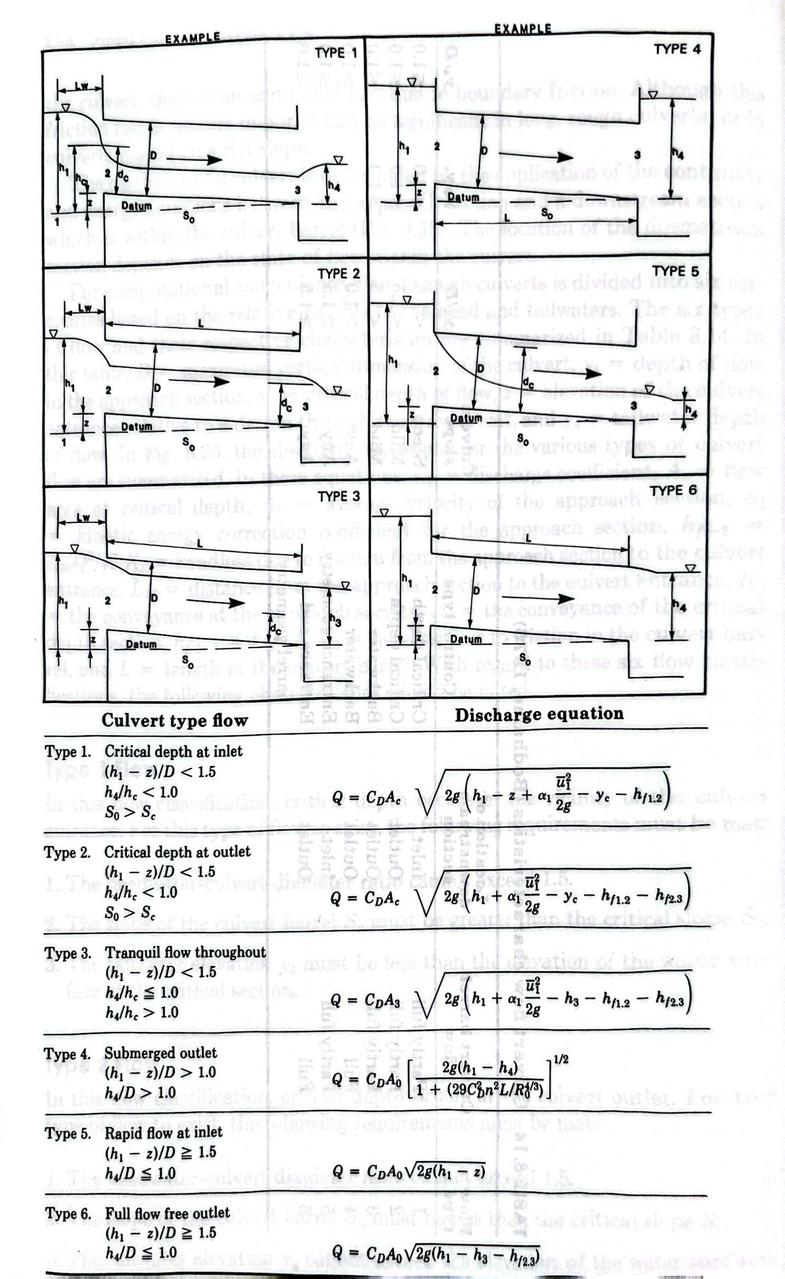
\includegraphics[width=0.8\linewidth]{fig826.jpeg}
    \caption{Tipos de flujo a trav\'es de un culvert (tomado de \cite{French}).}
    \label{fig826}
\end{figure}

En la figura~\ref{fig826} se presentan las curvas de caudal vs profundidad $Q=f(y)$ para cada uno de los tipos en donde $C_d$ es el coeficiente de descarga, $A_c$ es el area para la profundidad cr\'itica, $\bar{u_1}$ velocidad promedio aguas arriba, $\alpha_1$ coeficiente de energ\'ia cin\'etica para la velocidad aguas arriba, $h_{f_{1-2}} = \frac{L_w Q^2}{K_1 K_c}$ es la p\'erdida de energi\'ia desde una secci\'on aguas arriba hasta la secci\'on de entrada al culvert, $L_w$ es la distancia desde la secci\'on aguas arriba hasta la entrada, $K_1$ es el factor de secci\'on $\frac{C_o}{n} A R^{2/3}$ en la secci\'on aguas arriba, $K_c$ es el factor de secci\'on para $y_c$, $h_{f_{2-3}} = \frac{L Q^2}{K_2 K_3}$ es la p\'erdida de energi\'ia lo largo del culvert, y $L$ es la longitud del culvert. 

\subsection*{Flujo tipo 1}
$y_c$ ocurre a la entrada del culvert. Para que este flujo ocurra, se debe cumplir:
\begin{itemize}
    \item $y_1/D < 1.5$ 
    \item $S_o > S_c$
    \item $h_4 < y_c$
\end{itemize}

\subsection*{Flujo tipo 2}
$y_c$ ocurre a la salida del culvert. Para que este flujo ocurra, se debe cumplir:
\begin{itemize}
    \item $y_1/D < 1.5$ 
    \item $S_o < S_c$
    \item $h_4 < y_c$
\end{itemize}

\subsection*{Flujo tipo 3}
Ocurre flujo gradualmente variado a lo largo del culvert y el flujo es subcr\'itico. Para que este flujo ocurra, se debe cumplir:
\begin{itemize}
    \item $y_1/D < 1.5$ 
    \item $h_4 > y_c$ 
\end{itemize}

\subsection*{Flujo tipo 4}
El culvert trabaja a presi\'on y el caudal se puede estimar al aplicar la ecuaci\'on de energ\'ia entre las secciones aguas arriba y aguas abajo. Las p\'erdidas de energ\'ia a la entrada y a lo largo del culvert se desprecian usualmente. Las p\'erdidas debido a la expansi\'on a la salida se calcula como $h_3 - h_4$ 

\subsection*{Flujo tipo 5}
El flujo es supercr\'itico y $y_1/D >= 1.5$. 


\subsection*{Flujo tipo 6}
En este flujo $y_1/D >= 1.5$, el culvert luce lleno pero la salida del culvert no esta sumergida.  

Para calcular el caudal que pasa a traves del culvert, es necesario definir el $n$ de Manning que depende del material y del di\'ametro del culvert (ver tablas ~\ref{tab1}, ~\ref{tab2} y ~\ref{tab3}).
% French tab 8.16
\begin{table}[h!]
\centering
\begin{tabular}{c c}
 \hline
 Diameter (ft) & Manning's $n$ \\ [0.5ex]
 \hline\hline
 1 & 0.027 \\
 2 & 0.025 \\
 3-4 & 0.024 \\
 5-7 & 0.023 \\
 8 & 0.022 \\
\hline
\end{tabular}
\caption{Coeficientes de rugosidad de Manning para acero corrugado estandard (tomado de \cite{French}).}
\label{tab1}
\end{table}

% French tab 8.17
\begin{table}[h!]
\centering
\begin{tabular}{c c}
 \hline
 Diameter (ft) & Manning's $n$ \\ [0.5ex]
 \hline\hline
 5-6 & 0.034 \\
 7-8 & 0.033 \\
 9-11 & 0.032 \\
 12-13 & 0.031 \\
 14-15 & 0.030 \\
 16-18 & 0.029 \\
 19-20 & 0.028 \\
 21-22 & 0.027 \\
\hline
\end{tabular}
\caption{Coeficientes de rugosidad de Manning para culvert en acero construido en sitio (tomado de \cite{French}).}
\label{tab2}
\end{table}

% French tab 8.18
\begin{table}[h!]
\centering
\begin{tabular}{c c}
 \hline
 Concrete conditions (ft) & Manning's $n$ \\ [0.5ex]
 \hline\hline
 Very smooth & 0.010 \\
 Smooth & 0.011-0.015 \\
 Ordinary field construction & 0.012-0.015 \\
 Badly spalled & 0.015-0.020 \\
\hline
\end{tabular}
\caption{Coeficientes de rugosidad de Manning para culverts en concreto (tomado de \cite{French}).}
\label{tab3}
\end{table}

La determinaci\'on de $C_d$, se ha realizado a trav\'es de ensayos de laboratorio. $C_d$ depende de la forma y tamaño de la entrada al box culvert. Para determinar su valor, se ha agrupado el tipo de flujo a trav\'es del culvert de la siguiente manera:

\begin{itemize}
    \item \emph{Flujos 1, 2 y 3}: El valor de $C_d$ para entradas bruscas (cuadradas) se obtiene con base en $y_1/D$ (ver figura~\ref{fig827}). Sin embargo, el valor de $C_d$ se debe corregir por un factor que depende de la forma de la entrada. Se multiplica por $k_r$ para entradas redondeadas (ver figura~\ref{fig828}) y por $k_w$ para entradas con transici\'on (ver figura~\ref{fig829}).
% French fig 8-27
\begin{figure}[h]
    \centering
    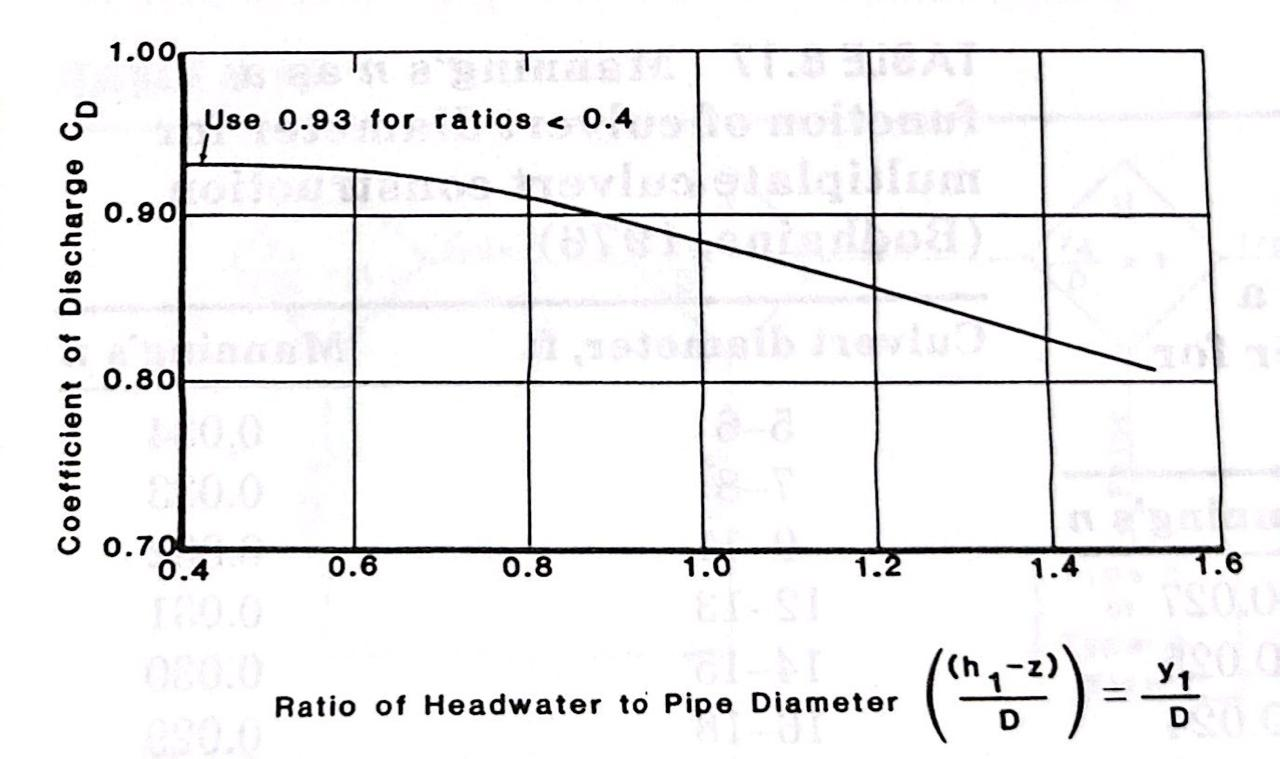
\includegraphics[width=0.8\linewidth]{fig827.jpeg}
    \caption{Valores de $C_d$ para flujos tipo 1, 2 y 3 en culverts (tomado de \cite{French}).}
    \label{fig827}
\end{figure}
% French fig 8-28
\begin{figure}[h]
    \centering
    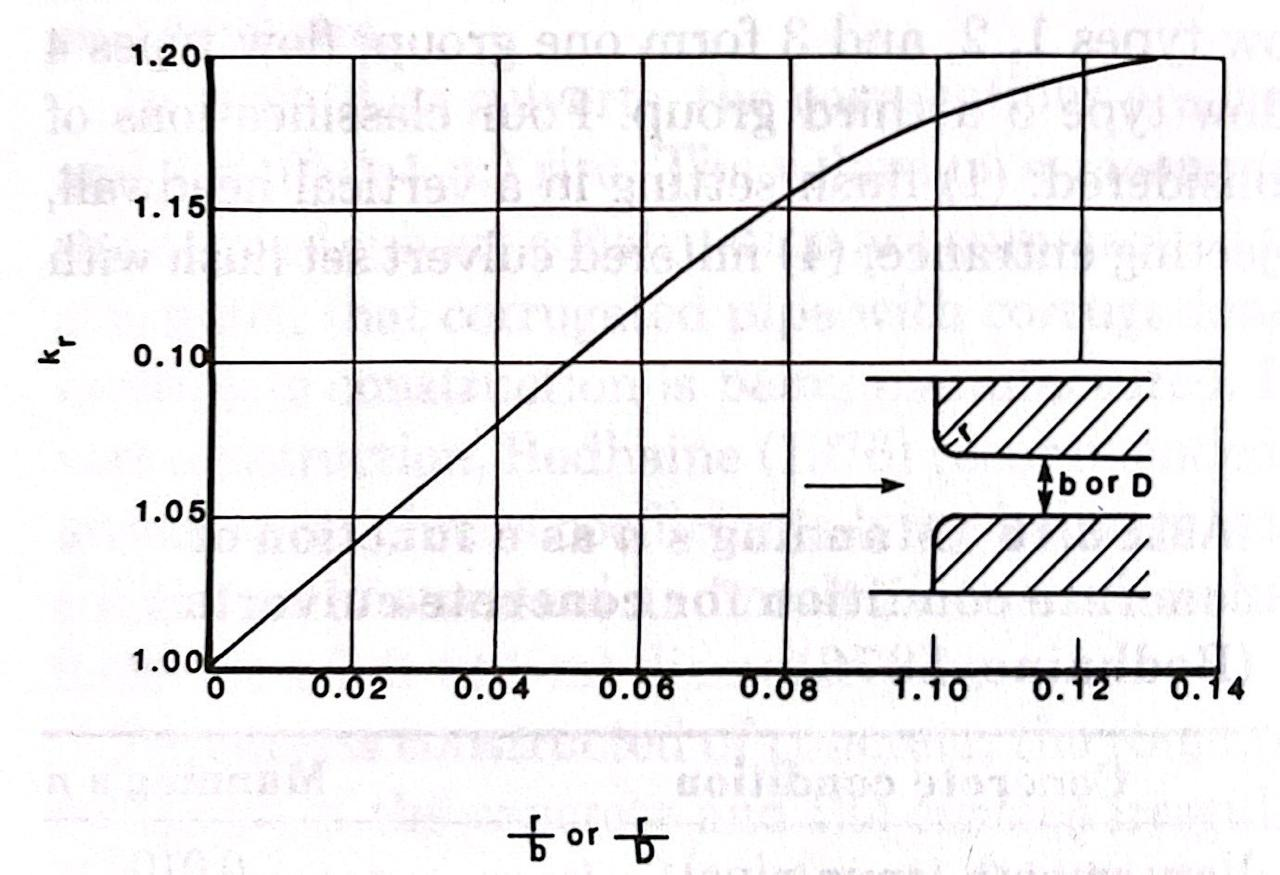
\includegraphics[width=0.8\linewidth]{fig828.jpeg}
    \caption{Valores de $k_r$ para entradas redondeadas (tomado de \cite{French}).}
    \label{fig828}
\end{figure}
% French fig 8-29
\begin{figure}[h]
    \centering
    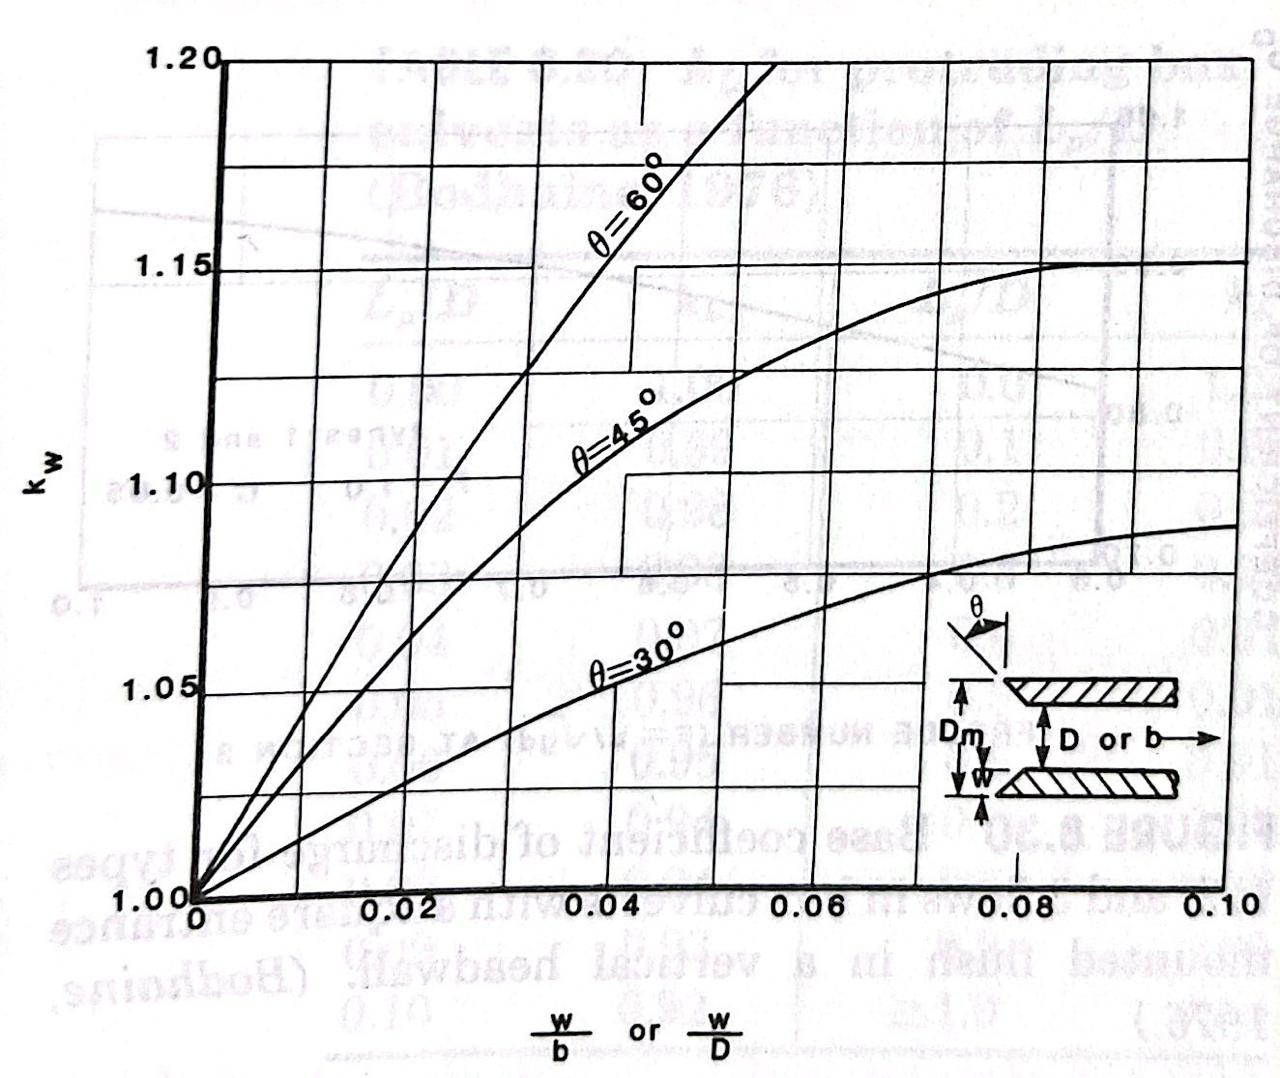
\includegraphics[width=0.8\linewidth]{fig829.jpeg}
    \caption{Valores de $k_w$ para entradas en transici\'on (tomado de \cite{French}).}
    \label{fig829}
\end{figure}

$C_d$ tambi\'en puede ser obtenido de graficas a partir del numero de Froude a la salida del culvert (secci\'on 3). $C_d$ debe ser corregido dependiendo de la forma de la entrada al culvert. 

\item \emph{Flujos 4 y 6}: $C_d$ puede ser estimado con base en la tabla~\ref{tab4}. 
% French tab 8.21
\begin{table}[h!]
\centering
\begin{tabular}{c c}
 \hline
 $r/b$, $w/b$, $w/D$ o $r/D$ & $C_d$ \\ [0.5ex]
 \hline\hline
 0 & 0.84 \\
 0.02 & 0.88 \\
 0.04 & 0.91 \\
 0.06 & 0.94 \\
 0.08 & 0.96 \\
 0.10 & 0.97 \\
 0.12 & 0.98 \\
\hline
\end{tabular}
\caption{$C_d$ para flujo tipo 4 y 6 en un culvert (tomado de \cite{French}).}
\label{tab4}
\end{table}

Con base en la forma de la entrada, los valores de $C_d$ tambi\'en se puede establecer. 

\item \emph{Flujo tipo 5}: El valor de $C_d$ para culverts se puede determinar de la figura~\ref{fig822}.
% French tabla 8-22
\begin{figure}[h]
    \centering
    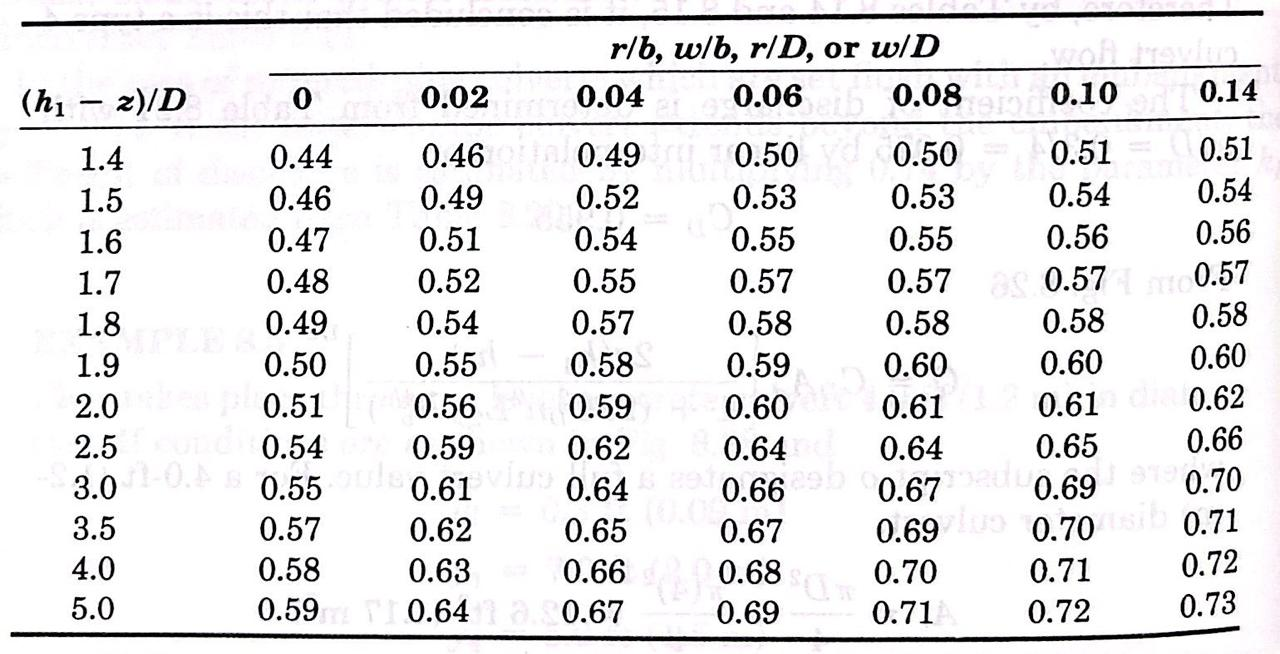
\includegraphics[width=0.8\linewidth]{fig822.jpeg}
    \caption{Valores de $C_d$ para culvert con flujo tipo 5 (tomado de \cite{French}).}
    \label{fig822}
\end{figure}

\end{itemize}


% REFERENCES
\bibliographystyle{plain} % We choose the "plain" reference style
\bibliography{refs} % Entries are in the refs.bib file

\end{document}
